The SPIKE distance \citep{KreuzEtAl2011a,KreuzEtAl2012a} which was introduced in Chapter One is a time-local parameter-free distance measure between spike-trains.  This measure can then be integrated over the length of the spike-trains to give a parameter-free distance measure between two spike trains.  

In the study of spike-train metrics, often a multi-unit measure is desired, as many data sets record several neurons at once.  A multi-unit measure is a distance between collections of labelled spike-trains.  The SPIKE distance in \citep{KreuzEtAl2011a} does not lend itself to a simple multi-unit extension, so instead a simpler version of the SPIKE distance is extended.

\section{Alternative SPIKE distance}
With a view to extending the SPIKE distance to a multi-unit distance measure, it is useful to review the definition of the SPIKE measure provided in \citep{KreuzEtAl2011a}:  Given two spike-trains $X$ and $Y$, where $x = \{ t_1^x, \ldots, t_n^x \}$ and $y = \{ t_1^y, \ldots , t_m^y\}$, where $t_1^x,\ldots,t_n^x,t_1^y,\ldots,t_m^y$ are the spike times.  The SPIKE distance in \citep{KreuzEtAl2011a} has the nice property that the distance is bounded such that it is always between zero and one.  Unfortunately, to achieve a natural extension to a multi-unit measure, this property is sacrificed.  A simpler version of the distance, without the strict upper bound of one, is used.

The simpler distance is very quick and easy to calculate.  A gap is associated with each spike; this is the distance to the nearest spike in the other spike-train.  The total distance between two spike trains is then simply the sum of these gaps.  

The original SPIKE distance included additional normalisation factors that have been omitted here. This simplifies the measure between complete spike trains greatly. The simpler measure is also provably a metric between spike trains. This measure is certainly symmetric and non-negative, and the triangle inequality holds due the $L^1$ metric.

To form the time-local distance, a weighted sum of the gaps for the corner spikes is made, that is, the spikes preceding and following the time of interest in each of the two spike trains.  The weighting is chosen so that the integral of the time-local function is just the sum of the gaps.

First, the gaps are calculated for each spike in the two spike-trains.  This is simply the nearest spike in the other spike train:
\begin{equation}
\Delta t_i^x = \min_i ( | t_i^x - t_i^y |)
\end{equation}
At each time instant, these is a unique set of four corner spikes: the preceding and following spikes from each spike train, which are labelled $t_P^x(t), t_F^x(t), t_P^y(t)$ and  $t_F^y(t)$; these are, respectively, the preceding and following spikes in spike-train $X$ and the preceding and following spikes in spike-train $Y$.

For each spike-train, $W\in \{ X, Y \}$, a time-local distance is then calculated using the associated gap of the four corner spikes for each spike-train, $w=x,y$:
\begin{equation}
s_w(t) = \frac{\lambda_P(t) \Delta t_P^w(t) + \lambda_F(t)\Delta t_F^w(t)}{I^w(t)}
\end{equation}
where
\begin{equation}
\begin{split}
\lambda_F^w(t) &= \frac{t- t_P^w(t)}{I^w(t)}\\ \lambda_P^w(t) &= \frac{ t_F^w(t) - t}{I^w(t)}
\end{split}
\end{equation}
and $I^w(t)$ is the size of the interval in which $t$ is contained:
\begin{equation}
I^w(t) = t_F^w(t) - t_P^w(t).
\end{equation}
Now, the time-local distance for each neuron is added to give the overall time-local distance:
\begin{equation}
s(t) = s_x(t) + s_y(t).
\end{equation}

This simplified time-local SPIKE distance has the advantage that its integral is simply the sum of the gaps of each spike; that is:
\begin{equation}
\int_0^T s(t)\, dt = \sum_w \sum_i \Delta t_i^w.
\end{equation}

In practice this simplified version of SPIKE produces similar time profiles to the version described in \citep{KreuzEtAl2011a}.


\section{Extensions to multi-unit recordings}
As recording methods have improved, there are now more and more data sets recorded by multi-probe recordings.  These recordings can isolate many separate neurons simultaneously, but it is not clear how exactly these collections of spike-trains should be compared to each other.  Typically, there are two extreme cases for multi-unit recordings, and a population parameter is varied to find the best mix.  

The first extreme case would be where each neuron is carrying a completely independent signal to all the other neurons.  In this case, each spike-train from a specific neuron should only be compared to other spike-trains from the same neuron.  This is called a \emph{labelled line} (LL) code.  For a LL code, a spike train labelled $i$ will only be compared to other spike trains with the same label, and then the distances are summed over all the labels.

The second extreme case would be that all the neurons are carrying the same signal.  In this case, it would not make sense to only compare spike trains with the same label; it would be expected that the signal would be carried by the whole population.  This is called a \emph{summed population} (SP) code.  Typically for a SP code, the spike trains are all pooled together and they are then treated as one large spike train.

In \citep{HoughtonSen2008a}, the van Rossum metric which was introduced in Chapter One was extended to the multi-unit case, and in \citep{Aronovetal2003a} the Victor-Purpura metric was extended.  A multi-unit distance is defined to be between two sets of spike-trains; $\mathbf{X}=\{ X_i \}$ and $ \mathbf{Y}=\{ Y_i \}$, where $i \in 1\ldots N$ and the index $i$ labels the neuron.

The single-unit distance from the previous section is extended to a multi-unit distance. All that is required to calculate is the gap associated with each spike in each set of spike trains. By including the possibility that the nearest spike may belong to a different neuron in the other set, this is achieved. However there must a distance penalty associated with changing from one neuron to the other. This penalty is similar to the costs in edit-length metrics such as Victor-Purpura \citep{VictorPurpura1997a}. 

In other words, it is necessary to introduce a parameter $k$, which quantifies a fictional distance between spikes fired in different cells.  The size of this distance quantifies the importance of the labelling of the neurons, and varying $k$ interpolates smoothly from $k=0$, a summed population (SP) code, to $k$ large, a labeled line  (LL) code.  While theoretically the LL code occurs as $k \rightarrow \infty$, in practice a LL code occurs when $k$ is on the order of $2/\lambda$, where $\lambda$ is the average frequency of the trials.   The gaps can then be calculated as follows:

\begin{equation}\label{initspike}
\Delta t_{\alpha}^{x_i}(k) = \min_{\beta,j} \left( |t_{\alpha}^{x_i} - t_{\beta}^{y_j} | + k\left[1-\delta(i,j)\right] \right)
\end{equation}
where $\delta(i,j)$ is the Kroneker delta, which is one if $i$ and $j$ match and zero otherwise. Hence, if the spikes have the same label in $x$ and $y$ there is no added distance, otherwise $k$ is added to the time difference between the spikes.  This is illustrated in Figure \ref{fig:gaps2}

\begin{figure}[htb]
\begin{center}
\setlength{\unitlength}{.1cm}
\begin{picture}(100,40)

\linethickness{1.5pt}
\put(5,8.7){\mbox{$\mathbf{2}$}}
\put(5,28.7){\mbox{$\mathbf{1}$}}
\put(10,10){\line(1,0){80}}
\put(10,30){\line(1,0){80}}

\linethickness{1pt}
\put(85,20){\vector(0,1){10}}
\put(85,20){\vector(0,-1){10}}
\put(87,18.5){\mbox{$k$}}

\put(20,11){\line(0,1){2}}
\put(20,12){\line(1,0){5}}
\put(25,12){\vector(0,1){16}}

\put(25,31){\line(0,1){2}}
\put(30,32){\vector(1,0){10}}
\put(30,32){\vector(-1,0){5}}
\put(40,31){\line(0,1){2}}

\put(50,11){\line(0,1){2}}
\put(55,12){\vector(1,0){5}}
\put(55,12){\vector(-1,0){5}}
\put(60,11){\line(0,1){2}}

\put(65,31){\line(0,1){2}}
\put(70,32){\vector(1,0){5}}
\put(70,32){\vector(-1,0){5}}
\put(75,31){\line(0,1){2}}

\put(18.5,9.1){\mbox{{\bf$\times$}}}
\put(18.5,5){\mbox{{\bf e}}}
\put(58.5,9.1){\mbox{{\bf$\times$}}}
\put(58.5,5){\mbox{{\bf g}}}
\put(63.5,29.1){\mbox{{\bf$\times$}}}
\put(63.5,25){\mbox{{\bf c}}}
\put(38.5,29.1){\mbox{{\bf$\times$}}}
\put(38.5,25){\mbox{{\bf b}}}
\put(25,30){\circle{2}}
\put(21,25){\mbox{{\bf a}}}
\put(50,10){\circle{2}}
\put(48,5){\mbox{{\bf f}}}
\put(75,30){\circle{2}}
\put(73,25){\mbox{{\bf d}}}
\end{picture}
\end{center}
\bigskip
\rule{33em}{0.5pt}
\caption{\label{fig:gaps2}An example of how to calculate the gaps between spikes.  If  the circles represent spikes from $\mathbf{X}$ and crosses represent spikes from $\mathbf{Y}$, then in the picture above, the distance $k$ is simply the cost of relabelling a spike.  Spike {\bf e} in $Y_2$ is much closer to spike {\bf a} in $X_1$ than {\bf f} in $X_2$, so it pays the cost $k$ to get its $\Delta$ from {\bf a}.}
\end{figure}

The time-local distance measure is then defined as before, using the corner spikes normalised by the inter-spike-interval:
\begin{equation}
s_{\mathbf{X}}(t) = \sum_{\mathbf{x}_i \in \mathbf{X}} \frac{\lambda_{\mathrm{P}}(t)\Delta t_{\mathrm{P}}^{\mathbf{x}_i} (t) + \lambda_{\mathrm{F}}(t)\Delta t_{\mathrm{F}}^{\mathbf{x}_i}(t) }{I^{\mathbf{x}_i}(t) }%t_{\mathrm{F}}^{\mathbf{x}_i} - t_{\mathrm{P}}^{\mathbf{x}_i}}
\end{equation}
where 
\begin{equation}
\lambda_{\mathrm{F}}^{\mathbf{x}_i}(t) =\frac{ t-t_{\mathrm{P}}^{\mathbf{x}_i}(t)}{I^{\mathbf{x}_i}(t)}%t_{\mathrm{F}}^{\mathbf{x}_i}(t) - t_{\mathrm{P}}^{\mathbf{x}_i}(t)}
\end{equation}
and
\begin{equation}
 \lambda_{\mathrm{P}}^{\mathbf{x}_i}(t) =\frac{ t_{\mathrm{F}}^{\mathbf{x}_i}(t) - t}{I^{\mathbf{x}_i}(t)}%{t_{\mathrm{F}}^\mathbf{x}_i}(t) - t_{\mathrm{P}}^{\mathbf{x}_i}(t)}
\end{equation}
and $I^{\mathbf{x}_i}(t)$ is the length of the interval in the spike-train $\mathbf{x}_i$ containing $t$, $I^{\mathbf{x}_i}(t) = t_{\mathrm{F}}^{\mathbf{x}_i}(t) - t_{\mathrm{P}}^{\mathbf{x}_i}(t)$.
 As before:
\begin{equation}
s(t) = s_{\mathbf{X}}(t) + s_{\mathbf{Y}}(t)
\end{equation}

Once more, this distance measure has the nice property that if the time-local measure is integrated over the course of the trial it equals the sum of the gaps of each spike:
\begin{equation}
\int_0^T s(t)\,dt = \sum_{\mathbf{W}} \sum_{\mathbf{w}_i \in \mathbf{W}} \sum_{\alpha} \Delta t_{\alpha}^{\mathbf{w}_i}
\end{equation}

While this extension seems like the most natural extension of the altered SPIKE distance measure, it does not have a clear boundary for when it becomes an LL code.  It appears that the distance stabilises at approximately twice the reciprocal of the rate, $2/r$, but this is not a precise bound.  If $2/r$ is the upper bound, then that would give a nice symmetry to the upper bound for the translation of spikes in the Victor-Purpura metric, as was mentioned in the introduction.

Motivated by \citep{HoughtonSen2008a}, another variant on the SPIKE extension was created.  \citet{HoughtonSen2008a} used geometry to compare the rate functions by rotating the vectors from perpendicular to parallel.  Since the SPIKE metric is an $L^1$ metric, any rotations must be along the $n-1$ simplex in $\mathbb{R}^n$.

A simplex is a convex mathematical object in $\mathbb{R}^n$, which is defined as all points $(a_1,\dots,a_n)$, such that $\sum_i a_i = 1$, and all $a_i\geq0$.  The $1$-simplex is a line in $\mathbb{R}^2$, the $2$-simplex is a triangle in $\mathbb{R}^3$ and the $3$-simplex is a tetrahedron in $\mathbb{R}^4$.

If each label $i$ is initially positioned at the $i$th unit vector, $(0,\ldots,1,\dots,0)$, then all the labels should travel along the simplex and meet at the centroid, $(1/n,\ldots,1/n)$.

A way to use this geometry could be by dividing the distances between labels $i$ and $j$ by the $j$th coordinate of label $i$ on the simplex.  That is:
\begin{equation}\label{multspike}
\Delta t_{\alpha}^{x_i}(p) = \left\{ \begin{array}{ll} \min_{\beta} | t_{\alpha}^{x_i} - t_{\beta}^{x_i} | & , \, p=0 \\
\min_{j,\beta}\left\{ \frac{n}{n-(n-1)p} | t_{\alpha}^{x_i} - t_{\beta}^{x_i} |,\frac{n}{p} | t_{\alpha}^{x_i} - t_{\beta}^{x_j} |\right\} & , \, 0<p\leq1 \end{array}\right.
\end{equation}

While this equation seems completely different to equation \ref{initspike} above, with a cost of $k$, this can actually be compared to it easily.  If the distance between labels is kept constant, then this equation becomes:
\begin{equation}
\Delta t_{\alpha}^{x_i}(p) = \left\{ \begin{array}{ll} \min_{\beta} | t_{\alpha}^{x_i} - t_{\beta}^{x_i} | & , \, p=0 \\
\min_{j,\beta}\left\{  | t_{\alpha}^{x_i} - t_{\beta}^{x_i} |,\left(1+\frac{n-pn}{p} \right) | t_{\alpha}^{x_i} - t_{\beta}^{x_j} |\right\} & , \, 0<p\leq1 \end{array}\right.
\end{equation}
So, there is an equivalence between $k$ and $p$, as follows:
\begin{equation}
k = \frac{n-pn}{n | t_{\alpha}^{x_i} - t_{\beta}^{x_j} |}
\end{equation}
%
%\begin{figure}[hbt]
%\include{spikemaxvmin}
%\caption{Performance of the proposed distance measure for different values of the mixing parameter $a$.  For each value of the mixing parameter $a$ the average value of the Transmitted Information is calculated for different values of $k$.  The solid line shows the maximum value over $k$, and the dotted line is the minimum value.  This figure should be compared to Figure 3 in \citep{HoughtonSen2008}.\label{fig:spikeminmax} }
%\end{figure}

 \subsection{Testing on data}
% 
% \begin{figure}[thb]
%\include{spikebest}
%\caption{The relationship between $k$ and $a$.  For each value of $a$, the value of $k$ giving the highest Transmitted Information is calculated over 20 runs.  The average is plotted, along with error bars representing the standard deviation.\label{fig:bestk}}
%\end{figure}

\begin{figure}[htb]
% GNUPLOT: LaTeX picture with Postscript
\begingroup
  \makeatletter
  \providecommand\color[2][]{%
    \GenericError{(gnuplot) \space\space\space\@spaces}{%
      Package color not loaded in conjunction with
      terminal option `colourtext'%
    }{See the gnuplot documentation for explanation.%
    }{Either use 'blacktext' in gnuplot or load the package
      color.sty in LaTeX.}%
    \renewcommand\color[2][]{}%
  }%
  \providecommand\includegraphics[2][]{%
    \GenericError{(gnuplot) \space\space\space\@spaces}{%
      Package graphicx or graphics not loaded%
    }{See the gnuplot documentation for explanation.%
    }{The gnuplot epslatex terminal needs graphicx.sty or graphics.sty.}%
    \renewcommand\includegraphics[2][]{}%
  }%
  \providecommand\rotatebox[2]{#2}%
  \@ifundefined{ifGPcolor}{%
    \newif\ifGPcolor
    \GPcolorfalse
  }{}%
  \@ifundefined{ifGPblacktext}{%
    \newif\ifGPblacktext
    \GPblacktexttrue
  }{}%
  % define a \g@addto@macro without @ in the name:
  \let\gplgaddtomacro\g@addto@macro
  % define empty templates for all commands taking text:
  \gdef\gplbacktext{}%
  \gdef\gplfronttext{}%
  \makeatother
  \ifGPblacktext
    % no textcolor at all
    \def\colorrgb#1{}%
    \def\colorgray#1{}%
  \else
    % gray or color?
    \ifGPcolor
      \def\colorrgb#1{\color[rgb]{#1}}%
      \def\colorgray#1{\color[gray]{#1}}%
      \expandafter\def\csname LTw\endcsname{\color{white}}%
      \expandafter\def\csname LTb\endcsname{\color{black}}%
      \expandafter\def\csname LTa\endcsname{\color{black}}%
      \expandafter\def\csname LT0\endcsname{\color[rgb]{1,0,0}}%
      \expandafter\def\csname LT1\endcsname{\color[rgb]{0,1,0}}%
      \expandafter\def\csname LT2\endcsname{\color[rgb]{0,0,1}}%
      \expandafter\def\csname LT3\endcsname{\color[rgb]{1,0,1}}%
      \expandafter\def\csname LT4\endcsname{\color[rgb]{0,1,1}}%
      \expandafter\def\csname LT5\endcsname{\color[rgb]{1,1,0}}%
      \expandafter\def\csname LT6\endcsname{\color[rgb]{0,0,0}}%
      \expandafter\def\csname LT7\endcsname{\color[rgb]{1,0.3,0}}%
      \expandafter\def\csname LT8\endcsname{\color[rgb]{0.5,0.5,0.5}}%
    \else
      % gray
      \def\colorrgb#1{\color{black}}%
      \def\colorgray#1{\color[gray]{#1}}%
      \expandafter\def\csname LTw\endcsname{\color{white}}%
      \expandafter\def\csname LTb\endcsname{\color{black}}%
      \expandafter\def\csname LTa\endcsname{\color{black}}%
      \expandafter\def\csname LT0\endcsname{\color{black}}%
      \expandafter\def\csname LT1\endcsname{\color{black}}%
      \expandafter\def\csname LT2\endcsname{\color{black}}%
      \expandafter\def\csname LT3\endcsname{\color{black}}%
      \expandafter\def\csname LT4\endcsname{\color{black}}%
      \expandafter\def\csname LT5\endcsname{\color{black}}%
      \expandafter\def\csname LT6\endcsname{\color{black}}%
      \expandafter\def\csname LT7\endcsname{\color{black}}%
      \expandafter\def\csname LT8\endcsname{\color{black}}%
    \fi
  \fi
  \setlength{\unitlength}{0.0500bp}%
  \begin{picture}(7200.00,5040.00)%
    \gplgaddtomacro\gplbacktext{%
      \csname LTb\endcsname%
      \put(1078,767){\makebox(0,0)[r]{\strut{} 0}}%
      \put(1078,1356){\makebox(0,0)[r]{\strut{} 0.25}}%
      \put(1078,1946){\makebox(0,0)[r]{\strut{} 0.5}}%
      \put(1078,2535){\makebox(0,0)[r]{\strut{} 0.75}}%
      \put(1078,3125){\makebox(0,0)[r]{\strut{} 1}}%
      \put(1078,3714){\makebox(0,0)[r]{\strut{} 1.25}}%
      \put(1078,4303){\makebox(0,0)[r]{\strut{} 1.5}}%
      \put(1210,484){\makebox(0,0){\strut{} 0}}%
      \put(2329,484){\makebox(0,0){\strut{} 0.1}}%
      \put(3447,484){\makebox(0,0){\strut{} 0.2}}%
      \put(4566,484){\makebox(0,0){\strut{} 0.3}}%
      \put(5684,484){\makebox(0,0){\strut{} 0.4}}%
      \put(6803,484){\makebox(0,0){\strut{} 0.5}}%
      \put(176,2771){\makebox(0,0){\strut{}$h$}}%
      \put(4006,154){\makebox(0,0){\strut{}$a$}}%
    }%
    \gplgaddtomacro\gplfronttext{%
    }%
    \gplbacktext
    \put(0,0){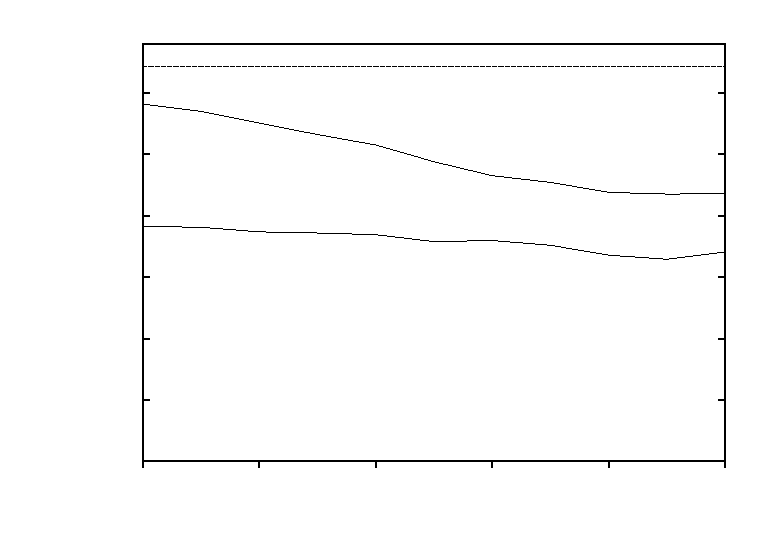
\includegraphics{BS}}%
    \gplfronttext
  \end{picture}%
\endgroup

\bigskip
\rule{33em}{0.5pt}
\caption{This figure shows the performance of the multi-unit SPIKE extension in identifying stimuli correctly in the data set described above.  The plot shows the maximum and minimum values of the transmitted information for each value of the mixing parameter $a$, averaged over 20 trials. This compares favourably with Figure 3 in \citep{HoughtonSen2008a}.}
\end{figure}

 The new extended measures were tested on the \citep{HoughtonSen2008a} test data as described in Chapter One. Two Poisson neurons form a receptive field and are each connected to two leaky integrate-and-fire neurons (LIF) with relative strength $a$ and $1-a$.  Hence, for $a=0$ each receptive neuron is connected to a single LIF neuron, and for $a=0.5$, each LIF neuron receives input equally from each of the receptive neurons.
 
  \begin{figure}[htb]
% GNUPLOT: LaTeX picture with Postscript
\begingroup
  \makeatletter
  \providecommand\color[2][]{%
    \GenericError{(gnuplot) \space\space\space\@spaces}{%
      Package color not loaded in conjunction with
      terminal option `colourtext'%
    }{See the gnuplot documentation for explanation.%
    }{Either use 'blacktext' in gnuplot or load the package
      color.sty in LaTeX.}%
    \renewcommand\color[2][]{}%
  }%
  \providecommand\includegraphics[2][]{%
    \GenericError{(gnuplot) \space\space\space\@spaces}{%
      Package graphicx or graphics not loaded%
    }{See the gnuplot documentation for explanation.%
    }{The gnuplot epslatex terminal needs graphicx.sty or graphics.sty.}%
    \renewcommand\includegraphics[2][]{}%
  }%
  \providecommand\rotatebox[2]{#2}%
  \@ifundefined{ifGPcolor}{%
    \newif\ifGPcolor
    \GPcolorfalse
  }{}%
  \@ifundefined{ifGPblacktext}{%
    \newif\ifGPblacktext
    \GPblacktexttrue
  }{}%
  % define a \g@addto@macro without @ in the name:
  \let\gplgaddtomacro\g@addto@macro
  % define empty templates for all commands taking text:
  \gdef\gplbacktext{}%
  \gdef\gplfronttext{}%
  \makeatother
  \ifGPblacktext
    % no textcolor at all
    \def\colorrgb#1{}%
    \def\colorgray#1{}%
  \else
    % gray or color?
    \ifGPcolor
      \def\colorrgb#1{\color[rgb]{#1}}%
      \def\colorgray#1{\color[gray]{#1}}%
      \expandafter\def\csname LTw\endcsname{\color{white}}%
      \expandafter\def\csname LTb\endcsname{\color{black}}%
      \expandafter\def\csname LTa\endcsname{\color{black}}%
      \expandafter\def\csname LT0\endcsname{\color[rgb]{1,0,0}}%
      \expandafter\def\csname LT1\endcsname{\color[rgb]{0,1,0}}%
      \expandafter\def\csname LT2\endcsname{\color[rgb]{0,0,1}}%
      \expandafter\def\csname LT3\endcsname{\color[rgb]{1,0,1}}%
      \expandafter\def\csname LT4\endcsname{\color[rgb]{0,1,1}}%
      \expandafter\def\csname LT5\endcsname{\color[rgb]{1,1,0}}%
      \expandafter\def\csname LT6\endcsname{\color[rgb]{0,0,0}}%
      \expandafter\def\csname LT7\endcsname{\color[rgb]{1,0.3,0}}%
      \expandafter\def\csname LT8\endcsname{\color[rgb]{0.5,0.5,0.5}}%
    \else
      % gray
      \def\colorrgb#1{\color{black}}%
      \def\colorgray#1{\color[gray]{#1}}%
      \expandafter\def\csname LTw\endcsname{\color{white}}%
      \expandafter\def\csname LTb\endcsname{\color{black}}%
      \expandafter\def\csname LTa\endcsname{\color{black}}%
      \expandafter\def\csname LT0\endcsname{\color{black}}%
      \expandafter\def\csname LT1\endcsname{\color{black}}%
      \expandafter\def\csname LT2\endcsname{\color{black}}%
      \expandafter\def\csname LT3\endcsname{\color{black}}%
      \expandafter\def\csname LT4\endcsname{\color{black}}%
      \expandafter\def\csname LT5\endcsname{\color{black}}%
      \expandafter\def\csname LT6\endcsname{\color{black}}%
      \expandafter\def\csname LT7\endcsname{\color{black}}%
      \expandafter\def\csname LT8\endcsname{\color{black}}%
    \fi
  \fi
  \setlength{\unitlength}{0.0500bp}%
  \begin{picture}(7200.00,5040.00)%
    \gplgaddtomacro\gplbacktext{%
      \csname LTb\endcsname%
      \put(1078,704){\makebox(0,0)[r]{\strut{} 0}}%
      \put(1078,1722){\makebox(0,0)[r]{\strut{} 0.05}}%
      \put(1078,2740){\makebox(0,0)[r]{\strut{} 0.1}}%
      \put(1078,3757){\makebox(0,0)[r]{\strut{} 0.15}}%
      \put(1078,4775){\makebox(0,0)[r]{\strut{} 0.2}}%
      \put(1676,484){\makebox(0,0){\strut{} 0}}%
      \put(2608,484){\makebox(0,0){\strut{} 0.1}}%
      \put(3540,484){\makebox(0,0){\strut{} 0.2}}%
      \put(4473,484){\makebox(0,0){\strut{} 0.3}}%
      \put(5405,484){\makebox(0,0){\strut{} 0.4}}%
      \put(6337,484){\makebox(0,0){\strut{} 0.5}}%
      \put(176,2739){\makebox(0,0){\strut{}$k$}}%
      \put(4006,154){\makebox(0,0){\strut{}$a$}}%
    }%
    \gplgaddtomacro\gplfronttext{%
    }%
    \gplbacktext
    \put(0,0){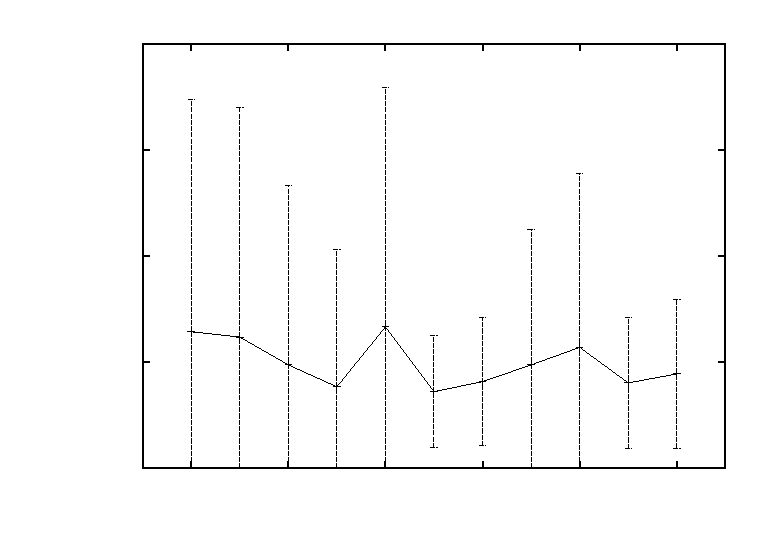
\includegraphics{bestBS}}%
    \gplfronttext
  \end{picture}%
\endgroup

\bigskip
\rule{33em}{0.5pt}
\caption{This figure shows the value for the penalty cost $k$ for the multi-unit SPIKE distance which gave the maximum transmitted information for each value of $a$.  There does not appear to be any trend towards LL or SP in either direction, the best value was always a mix of the two.}
\end{figure}

The maximum and minimum values of transmitted information, $h$, are then plotted against the mixing parameter $a$.  This allows comparison with the multi-unit van Rossum and multi-unit Victor-Purpura metrics which are plotted in \citep{HoughtonSen2008a}.
 
%
%\begin{figure}[htb]
%\include{spikeratio}
%\caption{The ratio of the transmitted information, $h$ of a labelled-line code (LL) and a summed-population code (SP).  For LL, $h$ is calculated for $k$ large, and for SP, $h$ is calculated for $k=0$. \label{fig:ratio}}
%\end{figure}
%\section{}
%\subsection{}
\begin{figure}[htb]
% GNUPLOT: LaTeX picture with Postscript
\begingroup
  \makeatletter
  \providecommand\color[2][]{%
    \GenericError{(gnuplot) \space\space\space\@spaces}{%
      Package color not loaded in conjunction with
      terminal option `colourtext'%
    }{See the gnuplot documentation for explanation.%
    }{Either use 'blacktext' in gnuplot or load the package
      color.sty in LaTeX.}%
    \renewcommand\color[2][]{}%
  }%
  \providecommand\includegraphics[2][]{%
    \GenericError{(gnuplot) \space\space\space\@spaces}{%
      Package graphicx or graphics not loaded%
    }{See the gnuplot documentation for explanation.%
    }{The gnuplot epslatex terminal needs graphicx.sty or graphics.sty.}%
    \renewcommand\includegraphics[2][]{}%
  }%
  \providecommand\rotatebox[2]{#2}%
  \@ifundefined{ifGPcolor}{%
    \newif\ifGPcolor
    \GPcolorfalse
  }{}%
  \@ifundefined{ifGPblacktext}{%
    \newif\ifGPblacktext
    \GPblacktexttrue
  }{}%
  % define a \g@addto@macro without @ in the name:
  \let\gplgaddtomacro\g@addto@macro
  % define empty templates for all commands taking text:
  \gdef\gplbacktext{}%
  \gdef\gplfronttext{}%
  \makeatother
  \ifGPblacktext
    % no textcolor at all
    \def\colorrgb#1{}%
    \def\colorgray#1{}%
  \else
    % gray or color?
    \ifGPcolor
      \def\colorrgb#1{\color[rgb]{#1}}%
      \def\colorgray#1{\color[gray]{#1}}%
      \expandafter\def\csname LTw\endcsname{\color{white}}%
      \expandafter\def\csname LTb\endcsname{\color{black}}%
      \expandafter\def\csname LTa\endcsname{\color{black}}%
      \expandafter\def\csname LT0\endcsname{\color[rgb]{1,0,0}}%
      \expandafter\def\csname LT1\endcsname{\color[rgb]{0,1,0}}%
      \expandafter\def\csname LT2\endcsname{\color[rgb]{0,0,1}}%
      \expandafter\def\csname LT3\endcsname{\color[rgb]{1,0,1}}%
      \expandafter\def\csname LT4\endcsname{\color[rgb]{0,1,1}}%
      \expandafter\def\csname LT5\endcsname{\color[rgb]{1,1,0}}%
      \expandafter\def\csname LT6\endcsname{\color[rgb]{0,0,0}}%
      \expandafter\def\csname LT7\endcsname{\color[rgb]{1,0.3,0}}%
      \expandafter\def\csname LT8\endcsname{\color[rgb]{0.5,0.5,0.5}}%
    \else
      % gray
      \def\colorrgb#1{\color{black}}%
      \def\colorgray#1{\color[gray]{#1}}%
      \expandafter\def\csname LTw\endcsname{\color{white}}%
      \expandafter\def\csname LTb\endcsname{\color{black}}%
      \expandafter\def\csname LTa\endcsname{\color{black}}%
      \expandafter\def\csname LT0\endcsname{\color{black}}%
      \expandafter\def\csname LT1\endcsname{\color{black}}%
      \expandafter\def\csname LT2\endcsname{\color{black}}%
      \expandafter\def\csname LT3\endcsname{\color{black}}%
      \expandafter\def\csname LT4\endcsname{\color{black}}%
      \expandafter\def\csname LT5\endcsname{\color{black}}%
      \expandafter\def\csname LT6\endcsname{\color{black}}%
      \expandafter\def\csname LT7\endcsname{\color{black}}%
      \expandafter\def\csname LT8\endcsname{\color{black}}%
    \fi
  \fi
  \setlength{\unitlength}{0.0500bp}%
  \begin{picture}(7200.00,5040.00)%
    \gplgaddtomacro\gplbacktext{%
      \csname LTb\endcsname%
      \put(1078,767){\makebox(0,0)[r]{\strut{} 0}}%
      \put(1078,1356){\makebox(0,0)[r]{\strut{} 0.25}}%
      \put(1078,1946){\makebox(0,0)[r]{\strut{} 0.5}}%
      \put(1078,2535){\makebox(0,0)[r]{\strut{} 0.75}}%
      \put(1078,3125){\makebox(0,0)[r]{\strut{} 1}}%
      \put(1078,3714){\makebox(0,0)[r]{\strut{} 1.25}}%
      \put(1078,4303){\makebox(0,0)[r]{\strut{} 1.5}}%
      \put(1210,484){\makebox(0,0){\strut{} 0}}%
      \put(2329,484){\makebox(0,0){\strut{} 0.1}}%
      \put(3447,484){\makebox(0,0){\strut{} 0.2}}%
      \put(4566,484){\makebox(0,0){\strut{} 0.3}}%
      \put(5684,484){\makebox(0,0){\strut{} 0.4}}%
      \put(6803,484){\makebox(0,0){\strut{} 0.5}}%
      \put(176,2771){\makebox(0,0){\strut{}$h$}}%
      \put(4006,154){\makebox(0,0){\strut{}$a$}}%
    }%
    \gplgaddtomacro\gplfronttext{%
    }%
    \gplbacktext
    \put(0,0){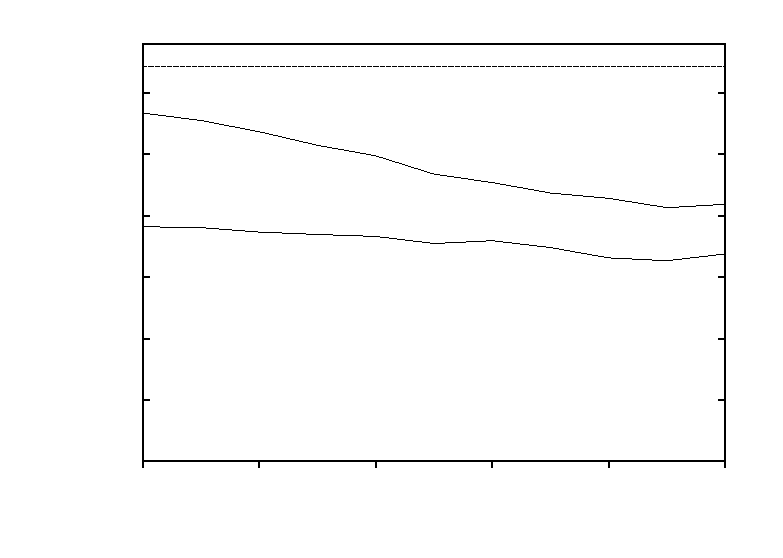
\includegraphics{multSPIKE}}%
    \gplfronttext
  \end{picture}%
\endgroup

\bigskip
\rule{33em}{0.5pt}
\caption{This figure shows the performance of the multiplicative multi-unit SPIKE extension, using the gaps from equation \ref{multspike}, in identifying stimuli correctly in the data set described above.  The plot shows the maximum and minimum values of the transmitted information for each value of the mixing parameter $a$, averaged over 20 trials.}
\end{figure}

\begin{figure}[htb]
\input{images/bestmultSpike}
\bigskip
\rule{33em}{0.5pt}
\caption{This figure shows the value for the population parameter $p$ for the multiplicative multi-unit SPIKE distance which gave the maximum transmitted information for each value of $a$.  There does not appear to be any trend towards LL or SP in either direction.}
\end{figure}

\newpage
\section{ISI distance}
\bigskip
\subsection{Single unit recordings}

With a view to extending the ISI distance to a multi-unit distance measure, it is useful to review the previous definition of the ISI distance between two spike trains $\mathbf{x}$ and $\mathbf{y}$ .  The ISI distance can be thought of as a rate-comparison, where the inter-spike interval (ISI) is used as a proxy for the firing rate.  As with all the time-local distance measures, it is defined as the interval over time of a local distance function $s(t)$.

Given two spike-trains $\mathbf{x}$ and $\mathbf{y}$, then $I^{\mathbf{x}}(t)$, $I^{\mathbf{y}}(t)$ are the inter-spike intervals at time $t$, for the spike-trains $\mathbf{x}$ and $\mathbf{y}$.  The time-local distance function is then defined in Kreuz et al. (2007) as:
\begin{equation}
s(t) = \left\{ \begin{array}{ll} 1-I^{\mathbf{x}}(t) / I^{\mathbf{y}}(t)  & \text{if } I^{\mathbf{x}}(t) \leq I^{\mathbf{y}}(t) \\ 1- I^{\mathbf{y}}(t) / I^{\mathbf{x}}(t)  & \text{otherwise} \end{array} \right.
\end{equation}
From the point of view of generalising to more than one neuron, it is convenient to rewrite this as:
\begin{equation}
s(t) = \frac{ | I^{\mathbf{x}}(t) - I^{\mathbf{y}}(t) | }{\max (I^{\mathbf{x}}(t), I^{\mathbf{y}}(t)) }
\end{equation}

\subsection{Initial extension to multi-unit recordings}

In the multi-unit case a distance is defined to be between two multi-unit recordings.  Thus, rather than two spike-trains there are two sets of spike-trains; $\mathbf{X}=\{ \mathbf{x}_i \}$ and $ \mathbf{Y}=\{ \mathbf{y}_i \}$, where $i \in 1\ldots N$ and the index $i$ is labelling the neuron.

The ISI-distance is a rate-based metric, so here a similar approach to multi-unit recordings as was used successfully for the van Rossum metric, another metric calculated using estimated rates, is used.  That approach, outlined in \citep{HoughtonSen2008}, replaces the rate with a rate-vector in an $N$-dimensional space.  To do this, each neuron is assigned a unit vector describing its direction in the rate-space.  At a given time, this is multiplied by the estimated rate of the neuron to give a rate-vector. The population rate-vector is then the sum of individual rate-vectors for each of the neurons in the population.  

An $L^1$ norm, $| I^{\mathbf{x}}(t) - I^{\mathbf{y}}(t) | $, appears in the numerator of $s(t)$ in the single-unit case, so the natural extension of this idea to the multi-unit ISI-distance involves an $L^1$-structure on the $N$-dimensional space, which is the ISI-space in this case. In practice this means the individual vectors are unit vectors under the $L^1$-norm; so for example for $N=2$, one vector may be $(1,0)$ and the other one would be $(1-\alpha,\alpha)$.  The corresponding individual neuron ISI-vectors would then be: 
\begin{equation}
\mathbf{I}^{\mathbf{x}_1}(t)=\begin{pmatrix}I^{\mathbf{x}_1}(t)\\0\end{pmatrix}
\end{equation}
\begin{equation}
\mathbf{I}^{\mathbf{x}_2}(t) = \begin{pmatrix} (1-\alpha)I^{\mathbf{x}_2}(t)\\ \alpha I^{\mathbf{x}_2}(t)\end{pmatrix}.
\end{equation}
The overall population ISI-vector $\mathbf{I^x}(t) = \mathbf{I}^{\mathbf{x}_1}(t) + \mathbf{I}^{\mathbf{x}_2}(t)$:
\begin{equation}
\mathbf{I^X}(t) = \begin{pmatrix} I^{\mathbf{x}_1}(t) + I^{\mathbf{x}_2}(t) - \alpha I^{\mathbf{x}_2}(t) \\ \alpha I^{\mathbf{x}_2}(t) \end{pmatrix}
\end{equation}

It remains to extend the definition of $s(t)$ to ISI-vectors. It is proposed here that this should be:
\begin{equation}
s(t) = \frac{ \| \mathbf{I^X}(t) - \mathbf{I^Y}(t) \|_1 }{ \sum_i \max ( I^X_i, I^Y_i ) }
\end{equation}
where $I^X_i, \, I^Y_i$ are the $i$th components of $\mathbf{I^X}$ and $\mathbf{I^Y}$ respectively, and:
\begin{equation}
\| \mathbf{I^X}(t) - \mathbf{I^Y}(t) \|_1 = \sum_i | I^X_i - I^Y_i |
\end{equation}

One important property of any multi-unit distance measure is that it interpolates from the summed population (SP) code  to the labelled line (LL) code .  In the case of the labelled line code, it is necessary to consider what the result should be, for example in the Victor-Purpura metric the LL code is the sum of the distances of the individual neurons, whereas in the case of the van Rossum metric, the LL code is the Pythagorean sum of the distances.  Here the LL code corresponds to when the vectors are all perpendicular,   this is $\alpha=1$ in the $N=2$ example above.  Up to an overall $L^1$ rotation, this means that the individual ISI vectors will have a single non-zero component, and $s(t)$ is given by:
\begin{equation}
s(t) = \frac{\sum_i | I^{\mathbf{x}_i} (t)  - I^{\mathbf{y}_i}(t)|}{\sum_i \max (I^{\mathbf{x}_i},I^{\mathbf{y}_i})}
 \end{equation}
 Given the rational structure of the ISI-distance, this seems to be the natural structure for the LL code.  
Conversely, when all the vectors are parallel, the result is the SP code:
\begin{equation}
s(t) = \frac{| \sum_i I^{\mathbf{x}_i}(t) - \sum_i I^{\mathbf{y}_i}(t) |}{\max (\sum_i I^{\mathbf{x}_i}(t),\sum_i I^{\mathbf{y}_i}(t) )}
\end{equation}
in which, effectively, the ISIs are averaged across the population before being compared in the distance measure.
%
%\begin{figure}[bht]
%\begin{center}
%% GNUPLOT: LaTeX picture with Postscript
\begingroup
  \makeatletter
  \providecommand\color[2][]{%
    \GenericError{(gnuplot) \space\space\space\@spaces}{%
      Package color not loaded in conjunction with
      terminal option `colourtext'%
    }{See the gnuplot documentation for explanation.%
    }{Either use 'blacktext' in gnuplot or load the package
      color.sty in LaTeX.}%
    \renewcommand\color[2][]{}%
  }%
  \providecommand\includegraphics[2][]{%
    \GenericError{(gnuplot) \space\space\space\@spaces}{%
      Package graphicx or graphics not loaded%
    }{See the gnuplot documentation for explanation.%
    }{The gnuplot epslatex terminal needs graphicx.sty or graphics.sty.}%
    \renewcommand\includegraphics[2][]{}%
  }%
  \providecommand\rotatebox[2]{#2}%
  \@ifundefined{ifGPcolor}{%
    \newif\ifGPcolor
    \GPcolorfalse
  }{}%
  \@ifundefined{ifGPblacktext}{%
    \newif\ifGPblacktext
    \GPblacktexttrue
  }{}%
  % define a \g@addto@macro without @ in the name:
  \let\gplgaddtomacro\g@addto@macro
  % define empty templates for all commands taking text:
  \gdef\gplbacktext{}%
  \gdef\gplfronttext{}%
  \makeatother
  \ifGPblacktext
    % no textcolor at all
    \def\colorrgb#1{}%
    \def\colorgray#1{}%
  \else
    % gray or color?
    \ifGPcolor
      \def\colorrgb#1{\color[rgb]{#1}}%
      \def\colorgray#1{\color[gray]{#1}}%
      \expandafter\def\csname LTw\endcsname{\color{white}}%
      \expandafter\def\csname LTb\endcsname{\color{black}}%
      \expandafter\def\csname LTa\endcsname{\color{black}}%
      \expandafter\def\csname LT0\endcsname{\color[rgb]{1,0,0}}%
      \expandafter\def\csname LT1\endcsname{\color[rgb]{0,1,0}}%
      \expandafter\def\csname LT2\endcsname{\color[rgb]{0,0,1}}%
      \expandafter\def\csname LT3\endcsname{\color[rgb]{1,0,1}}%
      \expandafter\def\csname LT4\endcsname{\color[rgb]{0,1,1}}%
      \expandafter\def\csname LT5\endcsname{\color[rgb]{1,1,0}}%
      \expandafter\def\csname LT6\endcsname{\color[rgb]{0,0,0}}%
      \expandafter\def\csname LT7\endcsname{\color[rgb]{1,0.3,0}}%
      \expandafter\def\csname LT8\endcsname{\color[rgb]{0.5,0.5,0.5}}%
    \else
      % gray
      \def\colorrgb#1{\color{black}}%
      \def\colorgray#1{\color[gray]{#1}}%
      \expandafter\def\csname LTw\endcsname{\color{white}}%
      \expandafter\def\csname LTb\endcsname{\color{black}}%
      \expandafter\def\csname LTa\endcsname{\color{black}}%
      \expandafter\def\csname LT0\endcsname{\color{black}}%
      \expandafter\def\csname LT1\endcsname{\color{black}}%
      \expandafter\def\csname LT2\endcsname{\color{black}}%
      \expandafter\def\csname LT3\endcsname{\color{black}}%
      \expandafter\def\csname LT4\endcsname{\color{black}}%
      \expandafter\def\csname LT5\endcsname{\color{black}}%
      \expandafter\def\csname LT6\endcsname{\color{black}}%
      \expandafter\def\csname LT7\endcsname{\color{black}}%
      \expandafter\def\csname LT8\endcsname{\color{black}}%
    \fi
  \fi
  \setlength{\unitlength}{0.0500bp}%
  \begin{picture}(7200.00,5040.00)%
    \gplgaddtomacro\gplbacktext{%
      \csname LTb\endcsname%
      \put(1078,767){\makebox(0,0)[r]{\strut{} 0}}%
      \put(1078,1356){\makebox(0,0)[r]{\strut{} 0.25}}%
      \put(1078,1946){\makebox(0,0)[r]{\strut{} 0.5}}%
      \put(1078,2535){\makebox(0,0)[r]{\strut{} 0.75}}%
      \put(1078,3125){\makebox(0,0)[r]{\strut{} 1}}%
      \put(1078,3714){\makebox(0,0)[r]{\strut{} 1.25}}%
      \put(1078,4303){\makebox(0,0)[r]{\strut{} 1.5}}%
      \put(1210,484){\makebox(0,0){\strut{} 0}}%
      \put(2329,484){\makebox(0,0){\strut{} 0.1}}%
      \put(3447,484){\makebox(0,0){\strut{} 0.2}}%
      \put(4566,484){\makebox(0,0){\strut{} 0.3}}%
      \put(5684,484){\makebox(0,0){\strut{} 0.4}}%
      \put(6803,484){\makebox(0,0){\strut{} 0.5}}%
      \put(176,2771){\rotatebox{-270}{\makebox(0,0){\strut{}h}}}%
      \put(4006,154){\makebox(0,0){\strut{}alpha}}%
    }%
    \gplgaddtomacro\gplfronttext{%
    }%
    \gplbacktext
    \put(0,0){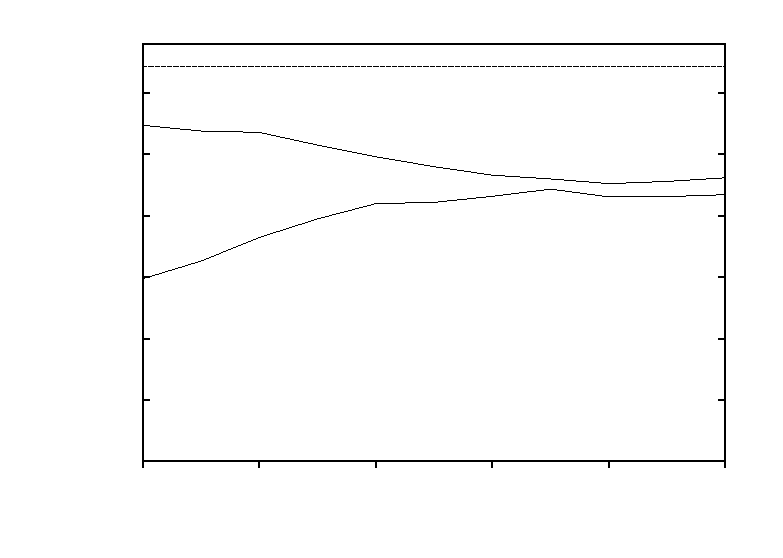
\includegraphics{maxmin}}%
    \gplfronttext
  \end{picture}%
\endgroup

%\end{center}
%\caption{Performance of the metric for different values of the mixing parameter $a$.  For each value of the mixing parameter $a$ the average value of the Transmitted Information is calculated for different values of $\alpha$.  The solid line shows the maximum value over $\alpha$, and the dotted line is the minimum value.  This figure should be compared to Figure 3 in \citep{HoughtonSen2008}.\label{fig:minmax}}
%\end{figure}
\begin{figure}[htb]
% GNUPLOT: LaTeX picture with Postscript
\begingroup
  \makeatletter
  \providecommand\color[2][]{%
    \GenericError{(gnuplot) \space\space\space\@spaces}{%
      Package color not loaded in conjunction with
      terminal option `colourtext'%
    }{See the gnuplot documentation for explanation.%
    }{Either use 'blacktext' in gnuplot or load the package
      color.sty in LaTeX.}%
    \renewcommand\color[2][]{}%
  }%
  \providecommand\includegraphics[2][]{%
    \GenericError{(gnuplot) \space\space\space\@spaces}{%
      Package graphicx or graphics not loaded%
    }{See the gnuplot documentation for explanation.%
    }{The gnuplot epslatex terminal needs graphicx.sty or graphics.sty.}%
    \renewcommand\includegraphics[2][]{}%
  }%
  \providecommand\rotatebox[2]{#2}%
  \@ifundefined{ifGPcolor}{%
    \newif\ifGPcolor
    \GPcolorfalse
  }{}%
  \@ifundefined{ifGPblacktext}{%
    \newif\ifGPblacktext
    \GPblacktexttrue
  }{}%
  % define a \g@addto@macro without @ in the name:
  \let\gplgaddtomacro\g@addto@macro
  % define empty templates for all commands taking text:
  \gdef\gplbacktext{}%
  \gdef\gplfronttext{}%
  \makeatother
  \ifGPblacktext
    % no textcolor at all
    \def\colorrgb#1{}%
    \def\colorgray#1{}%
  \else
    % gray or color?
    \ifGPcolor
      \def\colorrgb#1{\color[rgb]{#1}}%
      \def\colorgray#1{\color[gray]{#1}}%
      \expandafter\def\csname LTw\endcsname{\color{white}}%
      \expandafter\def\csname LTb\endcsname{\color{black}}%
      \expandafter\def\csname LTa\endcsname{\color{black}}%
      \expandafter\def\csname LT0\endcsname{\color[rgb]{1,0,0}}%
      \expandafter\def\csname LT1\endcsname{\color[rgb]{0,1,0}}%
      \expandafter\def\csname LT2\endcsname{\color[rgb]{0,0,1}}%
      \expandafter\def\csname LT3\endcsname{\color[rgb]{1,0,1}}%
      \expandafter\def\csname LT4\endcsname{\color[rgb]{0,1,1}}%
      \expandafter\def\csname LT5\endcsname{\color[rgb]{1,1,0}}%
      \expandafter\def\csname LT6\endcsname{\color[rgb]{0,0,0}}%
      \expandafter\def\csname LT7\endcsname{\color[rgb]{1,0.3,0}}%
      \expandafter\def\csname LT8\endcsname{\color[rgb]{0.5,0.5,0.5}}%
    \else
      % gray
      \def\colorrgb#1{\color{black}}%
      \def\colorgray#1{\color[gray]{#1}}%
      \expandafter\def\csname LTw\endcsname{\color{white}}%
      \expandafter\def\csname LTb\endcsname{\color{black}}%
      \expandafter\def\csname LTa\endcsname{\color{black}}%
      \expandafter\def\csname LT0\endcsname{\color{black}}%
      \expandafter\def\csname LT1\endcsname{\color{black}}%
      \expandafter\def\csname LT2\endcsname{\color{black}}%
      \expandafter\def\csname LT3\endcsname{\color{black}}%
      \expandafter\def\csname LT4\endcsname{\color{black}}%
      \expandafter\def\csname LT5\endcsname{\color{black}}%
      \expandafter\def\csname LT6\endcsname{\color{black}}%
      \expandafter\def\csname LT7\endcsname{\color{black}}%
      \expandafter\def\csname LT8\endcsname{\color{black}}%
    \fi
  \fi
  \setlength{\unitlength}{0.0500bp}%
  \begin{picture}(7200.00,5040.00)%
    \gplgaddtomacro\gplbacktext{%
      \csname LTb\endcsname%
      \put(1078,767){\makebox(0,0)[r]{\strut{} 0}}%
      \put(1078,1356){\makebox(0,0)[r]{\strut{} 0.25}}%
      \put(1078,1946){\makebox(0,0)[r]{\strut{} 0.5}}%
      \put(1078,2535){\makebox(0,0)[r]{\strut{} 0.75}}%
      \put(1078,3125){\makebox(0,0)[r]{\strut{} 1}}%
      \put(1078,3714){\makebox(0,0)[r]{\strut{} 1.25}}%
      \put(1078,4303){\makebox(0,0)[r]{\strut{} 1.5}}%
      \put(1210,484){\makebox(0,0){\strut{} 0}}%
      \put(2329,484){\makebox(0,0){\strut{} 0.1}}%
      \put(3447,484){\makebox(0,0){\strut{} 0.2}}%
      \put(4566,484){\makebox(0,0){\strut{} 0.3}}%
      \put(5684,484){\makebox(0,0){\strut{} 0.4}}%
      \put(6803,484){\makebox(0,0){\strut{} 0.5}}%
      \put(176,2771){\rotatebox{-270}{\makebox(0,0){\strut{}h}}}%
      \put(4006,154){\makebox(0,0){\strut{}alpha}}%
    }%
    \gplgaddtomacro\gplfronttext{%
    }%
    \gplbacktext
    \put(0,0){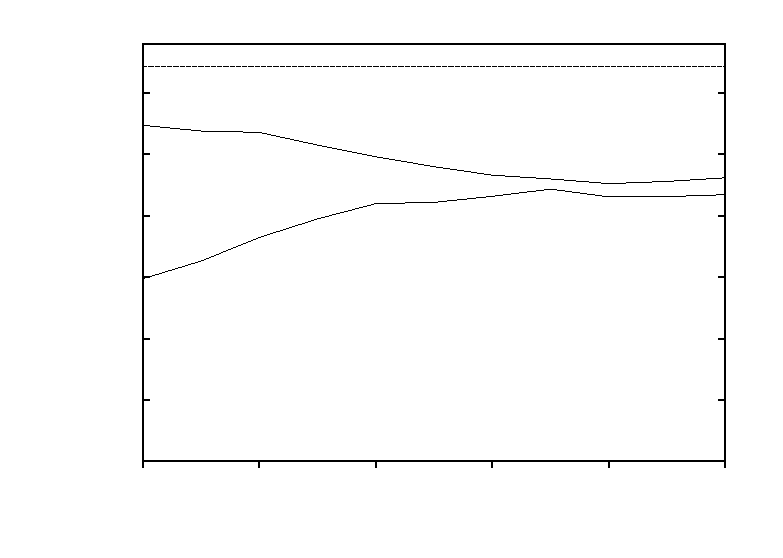
\includegraphics{maxmin}}%
    \gplfronttext
  \end{picture}%
\endgroup

\bigskip
\rule{33em}{0.5pt}
\caption{\label{mmav}The top line corresponds to the maximum possible transmitted information of $\log(5)$.  Then the upper of the two remaining lines is the average of the maximum transmitted information as $\alpha$ is varied from zero to a half, and the bottom line is the minimum transmitted information over $\alpha$.}
\end{figure}

\subsection{Numerical tests}
This multi-unit extension of the ISI distance is tested on the same data that was used above to test the multi-unit SPIKE distance. The ISI extension does not cluster the responses as well as the SPIKE extension when the mixing parameter $a$ is low, but it clusters the responses very well when the signals are more mixed.

While the extension proposed above was derived logically from the single-unit case, it does not agree with the standard definition of a summed-population code, that is, it is possible to find a population of neurons which have spiked at exactly the same time, but where the average inter-spike intervals are not equal at a given time.

\subsection{Alternative extensions to the multi-unit case}

Upon comparing the above extension to the previous extension to the multi-unit case by \citet{KreuzEtAl2009a}, it became clear that there was a fundamental difference in how each distance measure viewed the concept of a rate-based metric.


The extension proposed in \citep{KreuzEtAl2009a} interpolates between the average of the individual ISI distances and the ISI distance of the two ``population neurons'', that is, treating the individual spike times from the entire population as though they were all from the same neuron.  This is done with a ``population parameter'' $p$, which runs from $0$ (SP) to $1$ (LL).  This is given by:
\begin{equation}
\label{pop}
s_p(t) = (1-p)\left( \frac{ | I^{\mathbf{x}}(t) - I^{\mathbf{y}}(t) |}{ \max (I^{\mathbf{x}},I^{\mathbf{y}})}\right) + p\left( \frac{\sum_i | I^{\mathbf{x}_i}(t) - I^{\mathbf{y}_i}(t) |}{\sum_i \max (I^{\mathbf{x}_i},I^{\mathbf{y}_i})} \right),
\end{equation}
with notation as before, and $I^{\mathbf{x}}(t)$ is the interval in $\mathbf{x}$ at time $t$, where the population is viewed as a single neuron.

%\begin{figure}[thb]
%\begin{center}
%\input{images/popmaxvmin}
%\end{center}
%\caption{\label{popmaxmin}This is the performance of the extension proposed in the paper by Kreuz et al. \citep{Kreuzetal2009}.  The solid line represents the average of the maximum transmitted information ($h$) value across 20 trials, and the dotted line the minimum.  As we saw with the previous metric, the more the inputs are mixed, the more difficult it is to cluster the responses.}
%\end{figure}

The extension proposed above can be compared to the extension in \citep{KreuzEtAl2009a} by replacing the ISI of the ``population neuron'' with the average of the ISIs across the population of neurons.  This leads to the following equation: 
\begin{equation}
\label{av}
s_a(t) = (1-p) \left(\frac{ | \sum_i I^{\mathbf{x}_i}(t) - \sum_i I^{\mathbf{y}_i}(t) |}{\max (\sum_i I^{\mathbf{x}_i}(t),\sum_i I^{\mathbf{y}_i}(t) )}\right) + p\left( \frac{\sum_i | I^{\mathbf{x}_i}(t) - I^{\mathbf{y}_i}(t) |}{\sum_i \max (I^{\mathbf{x}_i},I^{\mathbf{y}_i})} \right),
\end{equation}.


\begin{figure}[htb]
% GNUPLOT: LaTeX picture with Postscript
\begingroup
  \makeatletter
  \providecommand\color[2][]{%
    \GenericError{(gnuplot) \space\space\space\@spaces}{%
      Package color not loaded in conjunction with
      terminal option `colourtext'%
    }{See the gnuplot documentation for explanation.%
    }{Either use 'blacktext' in gnuplot or load the package
      color.sty in LaTeX.}%
    \renewcommand\color[2][]{}%
  }%
  \providecommand\includegraphics[2][]{%
    \GenericError{(gnuplot) \space\space\space\@spaces}{%
      Package graphicx or graphics not loaded%
    }{See the gnuplot documentation for explanation.%
    }{The gnuplot epslatex terminal needs graphicx.sty or graphics.sty.}%
    \renewcommand\includegraphics[2][]{}%
  }%
  \providecommand\rotatebox[2]{#2}%
  \@ifundefined{ifGPcolor}{%
    \newif\ifGPcolor
    \GPcolorfalse
  }{}%
  \@ifundefined{ifGPblacktext}{%
    \newif\ifGPblacktext
    \GPblacktexttrue
  }{}%
  % define a \g@addto@macro without @ in the name:
  \let\gplgaddtomacro\g@addto@macro
  % define empty templates for all commands taking text:
  \gdef\gplbacktext{}%
  \gdef\gplfronttext{}%
  \makeatother
  \ifGPblacktext
    % no textcolor at all
    \def\colorrgb#1{}%
    \def\colorgray#1{}%
  \else
    % gray or color?
    \ifGPcolor
      \def\colorrgb#1{\color[rgb]{#1}}%
      \def\colorgray#1{\color[gray]{#1}}%
      \expandafter\def\csname LTw\endcsname{\color{white}}%
      \expandafter\def\csname LTb\endcsname{\color{black}}%
      \expandafter\def\csname LTa\endcsname{\color{black}}%
      \expandafter\def\csname LT0\endcsname{\color[rgb]{1,0,0}}%
      \expandafter\def\csname LT1\endcsname{\color[rgb]{0,1,0}}%
      \expandafter\def\csname LT2\endcsname{\color[rgb]{0,0,1}}%
      \expandafter\def\csname LT3\endcsname{\color[rgb]{1,0,1}}%
      \expandafter\def\csname LT4\endcsname{\color[rgb]{0,1,1}}%
      \expandafter\def\csname LT5\endcsname{\color[rgb]{1,1,0}}%
      \expandafter\def\csname LT6\endcsname{\color[rgb]{0,0,0}}%
      \expandafter\def\csname LT7\endcsname{\color[rgb]{1,0.3,0}}%
      \expandafter\def\csname LT8\endcsname{\color[rgb]{0.5,0.5,0.5}}%
    \else
      % gray
      \def\colorrgb#1{\color{black}}%
      \def\colorgray#1{\color[gray]{#1}}%
      \expandafter\def\csname LTw\endcsname{\color{white}}%
      \expandafter\def\csname LTb\endcsname{\color{black}}%
      \expandafter\def\csname LTa\endcsname{\color{black}}%
      \expandafter\def\csname LT0\endcsname{\color{black}}%
      \expandafter\def\csname LT1\endcsname{\color{black}}%
      \expandafter\def\csname LT2\endcsname{\color{black}}%
      \expandafter\def\csname LT3\endcsname{\color{black}}%
      \expandafter\def\csname LT4\endcsname{\color{black}}%
      \expandafter\def\csname LT5\endcsname{\color{black}}%
      \expandafter\def\csname LT6\endcsname{\color{black}}%
      \expandafter\def\csname LT7\endcsname{\color{black}}%
      \expandafter\def\csname LT8\endcsname{\color{black}}%
    \fi
  \fi
  \setlength{\unitlength}{0.0500bp}%
  \begin{picture}(7200.00,5040.00)%
    \gplgaddtomacro\gplbacktext{%
      \csname LTb\endcsname%
      \put(1078,767){\makebox(0,0)[r]{\strut{} 0}}%
      \put(1078,1356){\makebox(0,0)[r]{\strut{} 0.25}}%
      \put(1078,1946){\makebox(0,0)[r]{\strut{} 0.5}}%
      \put(1078,2535){\makebox(0,0)[r]{\strut{} 0.75}}%
      \put(1078,3125){\makebox(0,0)[r]{\strut{} 1}}%
      \put(1078,3714){\makebox(0,0)[r]{\strut{} 1.25}}%
      \put(1078,4303){\makebox(0,0)[r]{\strut{} 1.5}}%
      \put(1210,484){\makebox(0,0){\strut{} 0}}%
      \put(2329,484){\makebox(0,0){\strut{} 0.1}}%
      \put(3447,484){\makebox(0,0){\strut{} 0.2}}%
      \put(4566,484){\makebox(0,0){\strut{} 0.3}}%
      \put(5684,484){\makebox(0,0){\strut{} 0.4}}%
      \put(6803,484){\makebox(0,0){\strut{} 0.5}}%
      \put(176,2771){\rotatebox{-270}{\makebox(0,0){\strut{}h}}}%
      \put(4006,154){\makebox(0,0){\strut{}alpha}}%
    }%
    \gplgaddtomacro\gplfronttext{%
    }%
    \gplbacktext
    \put(0,0){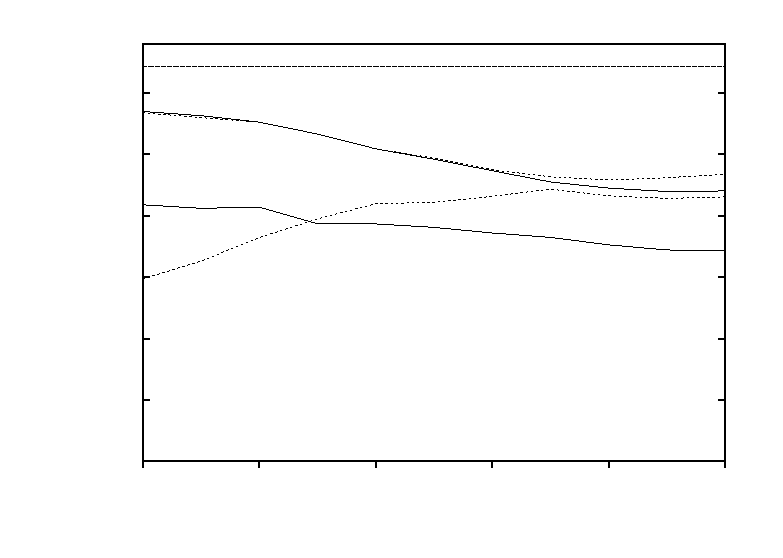
\includegraphics{avvspop}}%
    \gplfronttext
  \end{picture}%
\endgroup

\bigskip
\rule{33em}{0.5pt}
\caption{The lines, as in figure \ref{mmav} correspond to the maximum and the minimum for: $s_p$, the \lq{}population\rq{} extension, in the solid lines; and $s_a$, the \lq{}average\rq{} extension, in the broken lines.}
\end{figure}

\begin{figure}[htb]
% GNUPLOT: LaTeX picture with Postscript
\begingroup
  \makeatletter
  \providecommand\color[2][]{%
    \GenericError{(gnuplot) \space\space\space\@spaces}{%
      Package color not loaded in conjunction with
      terminal option `colourtext'%
    }{See the gnuplot documentation for explanation.%
    }{Either use 'blacktext' in gnuplot or load the package
      color.sty in LaTeX.}%
    \renewcommand\color[2][]{}%
  }%
  \providecommand\includegraphics[2][]{%
    \GenericError{(gnuplot) \space\space\space\@spaces}{%
      Package graphicx or graphics not loaded%
    }{See the gnuplot documentation for explanation.%
    }{The gnuplot epslatex terminal needs graphicx.sty or graphics.sty.}%
    \renewcommand\includegraphics[2][]{}%
  }%
  \providecommand\rotatebox[2]{#2}%
  \@ifundefined{ifGPcolor}{%
    \newif\ifGPcolor
    \GPcolorfalse
  }{}%
  \@ifundefined{ifGPblacktext}{%
    \newif\ifGPblacktext
    \GPblacktexttrue
  }{}%
  % define a \g@addto@macro without @ in the name:
  \let\gplgaddtomacro\g@addto@macro
  % define empty templates for all commands taking text:
  \gdef\gplbacktext{}%
  \gdef\gplfronttext{}%
  \makeatother
  \ifGPblacktext
    % no textcolor at all
    \def\colorrgb#1{}%
    \def\colorgray#1{}%
  \else
    % gray or color?
    \ifGPcolor
      \def\colorrgb#1{\color[rgb]{#1}}%
      \def\colorgray#1{\color[gray]{#1}}%
      \expandafter\def\csname LTw\endcsname{\color{white}}%
      \expandafter\def\csname LTb\endcsname{\color{black}}%
      \expandafter\def\csname LTa\endcsname{\color{black}}%
      \expandafter\def\csname LT0\endcsname{\color[rgb]{1,0,0}}%
      \expandafter\def\csname LT1\endcsname{\color[rgb]{0,1,0}}%
      \expandafter\def\csname LT2\endcsname{\color[rgb]{0,0,1}}%
      \expandafter\def\csname LT3\endcsname{\color[rgb]{1,0,1}}%
      \expandafter\def\csname LT4\endcsname{\color[rgb]{0,1,1}}%
      \expandafter\def\csname LT5\endcsname{\color[rgb]{1,1,0}}%
      \expandafter\def\csname LT6\endcsname{\color[rgb]{0,0,0}}%
      \expandafter\def\csname LT7\endcsname{\color[rgb]{1,0.3,0}}%
      \expandafter\def\csname LT8\endcsname{\color[rgb]{0.5,0.5,0.5}}%
    \else
      % gray
      \def\colorrgb#1{\color{black}}%
      \def\colorgray#1{\color[gray]{#1}}%
      \expandafter\def\csname LTw\endcsname{\color{white}}%
      \expandafter\def\csname LTb\endcsname{\color{black}}%
      \expandafter\def\csname LTa\endcsname{\color{black}}%
      \expandafter\def\csname LT0\endcsname{\color{black}}%
      \expandafter\def\csname LT1\endcsname{\color{black}}%
      \expandafter\def\csname LT2\endcsname{\color{black}}%
      \expandafter\def\csname LT3\endcsname{\color{black}}%
      \expandafter\def\csname LT4\endcsname{\color{black}}%
      \expandafter\def\csname LT5\endcsname{\color{black}}%
      \expandafter\def\csname LT6\endcsname{\color{black}}%
      \expandafter\def\csname LT7\endcsname{\color{black}}%
      \expandafter\def\csname LT8\endcsname{\color{black}}%
    \fi
  \fi
  \setlength{\unitlength}{0.0500bp}%
  \begin{picture}(7200.00,5040.00)%
    \gplgaddtomacro\gplbacktext{%
      \csname LTb\endcsname%
      \put(946,767){\makebox(0,0)[r]{\strut{} 0}}%
      \put(946,1569){\makebox(0,0)[r]{\strut{} 0.2}}%
      \put(946,2370){\makebox(0,0)[r]{\strut{} 0.4}}%
      \put(946,3172){\makebox(0,0)[r]{\strut{} 0.6}}%
      \put(946,3973){\makebox(0,0)[r]{\strut{} 0.8}}%
      \put(946,4775){\makebox(0,0)[r]{\strut{} 1}}%
      \put(1555,484){\makebox(0,0){\strut{} 0}}%
      \put(2509,484){\makebox(0,0){\strut{} 0.1}}%
      \put(3463,484){\makebox(0,0){\strut{} 0.2}}%
      \put(4418,484){\makebox(0,0){\strut{} 0.3}}%
      \put(5372,484){\makebox(0,0){\strut{} 0.4}}%
      \put(6326,484){\makebox(0,0){\strut{} 0.5}}%
      \put(176,2771){\rotatebox{-270}{\makebox(0,0){\strut{}p}}}%
      \put(3940,154){\makebox(0,0){\strut{}alpha}}%
    }%
    \gplgaddtomacro\gplfronttext{%
    }%
    \gplbacktext
    \put(0,0){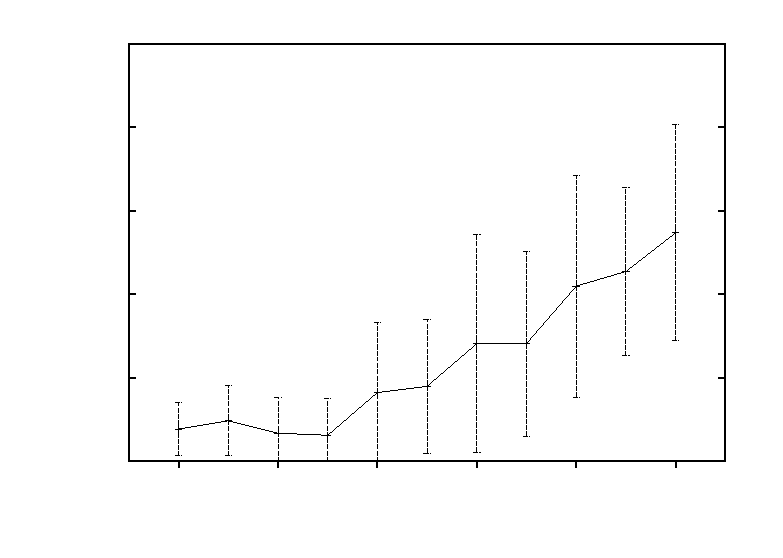
\includegraphics{bestpav}}%
    \gplfronttext
  \end{picture}%
\endgroup

\bigskip
\rule{33em}{0.5pt}
\caption{This figure shows the optimal value for the population parameter $p$ for $s_a$, the \lq{}average\rq{} extension, as the mixing parameter $a$ is varied from zero to a half, with the errorbars showing the standard deviation.}
\end{figure}

\begin{figure}[htb]
% GNUPLOT: LaTeX picture with Postscript
\begingroup
  \makeatletter
  \providecommand\color[2][]{%
    \GenericError{(gnuplot) \space\space\space\@spaces}{%
      Package color not loaded in conjunction with
      terminal option `colourtext'%
    }{See the gnuplot documentation for explanation.%
    }{Either use 'blacktext' in gnuplot or load the package
      color.sty in LaTeX.}%
    \renewcommand\color[2][]{}%
  }%
  \providecommand\includegraphics[2][]{%
    \GenericError{(gnuplot) \space\space\space\@spaces}{%
      Package graphicx or graphics not loaded%
    }{See the gnuplot documentation for explanation.%
    }{The gnuplot epslatex terminal needs graphicx.sty or graphics.sty.}%
    \renewcommand\includegraphics[2][]{}%
  }%
  \providecommand\rotatebox[2]{#2}%
  \@ifundefined{ifGPcolor}{%
    \newif\ifGPcolor
    \GPcolorfalse
  }{}%
  \@ifundefined{ifGPblacktext}{%
    \newif\ifGPblacktext
    \GPblacktexttrue
  }{}%
  % define a \g@addto@macro without @ in the name:
  \let\gplgaddtomacro\g@addto@macro
  % define empty templates for all commands taking text:
  \gdef\gplbacktext{}%
  \gdef\gplfronttext{}%
  \makeatother
  \ifGPblacktext
    % no textcolor at all
    \def\colorrgb#1{}%
    \def\colorgray#1{}%
  \else
    % gray or color?
    \ifGPcolor
      \def\colorrgb#1{\color[rgb]{#1}}%
      \def\colorgray#1{\color[gray]{#1}}%
      \expandafter\def\csname LTw\endcsname{\color{white}}%
      \expandafter\def\csname LTb\endcsname{\color{black}}%
      \expandafter\def\csname LTa\endcsname{\color{black}}%
      \expandafter\def\csname LT0\endcsname{\color[rgb]{1,0,0}}%
      \expandafter\def\csname LT1\endcsname{\color[rgb]{0,1,0}}%
      \expandafter\def\csname LT2\endcsname{\color[rgb]{0,0,1}}%
      \expandafter\def\csname LT3\endcsname{\color[rgb]{1,0,1}}%
      \expandafter\def\csname LT4\endcsname{\color[rgb]{0,1,1}}%
      \expandafter\def\csname LT5\endcsname{\color[rgb]{1,1,0}}%
      \expandafter\def\csname LT6\endcsname{\color[rgb]{0,0,0}}%
      \expandafter\def\csname LT7\endcsname{\color[rgb]{1,0.3,0}}%
      \expandafter\def\csname LT8\endcsname{\color[rgb]{0.5,0.5,0.5}}%
    \else
      % gray
      \def\colorrgb#1{\color{black}}%
      \def\colorgray#1{\color[gray]{#1}}%
      \expandafter\def\csname LTw\endcsname{\color{white}}%
      \expandafter\def\csname LTb\endcsname{\color{black}}%
      \expandafter\def\csname LTa\endcsname{\color{black}}%
      \expandafter\def\csname LT0\endcsname{\color{black}}%
      \expandafter\def\csname LT1\endcsname{\color{black}}%
      \expandafter\def\csname LT2\endcsname{\color{black}}%
      \expandafter\def\csname LT3\endcsname{\color{black}}%
      \expandafter\def\csname LT4\endcsname{\color{black}}%
      \expandafter\def\csname LT5\endcsname{\color{black}}%
      \expandafter\def\csname LT6\endcsname{\color{black}}%
      \expandafter\def\csname LT7\endcsname{\color{black}}%
      \expandafter\def\csname LT8\endcsname{\color{black}}%
    \fi
  \fi
  \setlength{\unitlength}{0.0500bp}%
  \begin{picture}(7200.00,5040.00)%
    \gplgaddtomacro\gplbacktext{%
      \csname LTb\endcsname%
      \put(946,767){\makebox(0,0)[r]{\strut{} 0}}%
      \put(946,1569){\makebox(0,0)[r]{\strut{} 0.2}}%
      \put(946,2370){\makebox(0,0)[r]{\strut{} 0.4}}%
      \put(946,3172){\makebox(0,0)[r]{\strut{} 0.6}}%
      \put(946,3973){\makebox(0,0)[r]{\strut{} 0.8}}%
      \put(946,4775){\makebox(0,0)[r]{\strut{} 1}}%
      \put(1555,484){\makebox(0,0){\strut{} 0}}%
      \put(2509,484){\makebox(0,0){\strut{} 0.1}}%
      \put(3463,484){\makebox(0,0){\strut{} 0.2}}%
      \put(4418,484){\makebox(0,0){\strut{} 0.3}}%
      \put(5372,484){\makebox(0,0){\strut{} 0.4}}%
      \put(6326,484){\makebox(0,0){\strut{} 0.5}}%
      \put(176,2771){\makebox(0,0){\strut{}$p$}}%
      \put(3940,154){\makebox(0,0){\strut{}$a$}}%
    }%
    \gplgaddtomacro\gplfronttext{%
    }%
    \gplbacktext
    \put(0,0){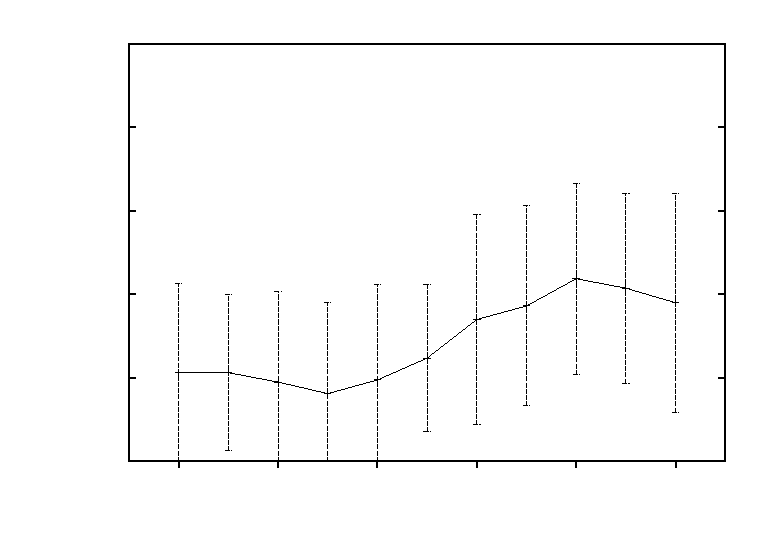
\includegraphics{bestppop}}%
    \gplfronttext
  \end{picture}%
\endgroup

\bigskip
\rule{33em}{0.5pt}
\caption{This figure shows the optimal value for the population parameter $p$ for $s_p$, the \lq{}population\rq{} extension, as the mixing parameter $a$ is varied from zero to a half, with the errorbars showing the standard deviation.}
\end{figure}
%\begin{figure}[htb]
%\begin{center}
%\include{newmaxvmin}
%\end{center}
%\caption{\label{avmaxmin} This is the performance of the alternative extension, using the average ISI, proposed here as a complementary measure. The solid line again represents the average of the maximum transmitted information across 20 trials, and the dotted lie the minimum.  The maximum is very comparable to the population ISI measure. The average ISI's minimum transmitted information performs worse when the signals are separate, and considerably better when the signals are mixed.}
%\end{figure}

There is a fundamental difference in how each of these distance measures view what a SP metric should be.  The example from \citep{KreuzEtAl2009a} assumes that there is information being carried by the frequency of arrival of spikes across the population, regardless of origin, and the second measure using the average ISI assumes that each neuron is essentially carrying the same message, with an inherent noise due to the biological constraints of neurons.  Each argument has its own merits, and it could be useful to have both of these measures, as in equations \ref{pop} and \ref{av}, depending on the focus of the experiment.


\newpage
\section{Adaptive ISI distances}

The downside to the measures introduced above is that there must be parameters to vary between the SP and LL cases, and thus far there is a way to choose a parameter, which often leads to a grid search to find the optimal parameter.  A goal of this work is to find a way for the data itself to choose its own population parameter.  The SPIKE and ISI distances for single neurons are both parameter-free, so it would be ideal if an extension could be found that was also parameter-free.

Since the ISI distance is a distance based on the firing rate of the neurons, the assumption was made that if the rates of the individual neurons were reasonably similar throughout the two populations, then the correct code to use would be an SP code, whereas if they were very different, then a LL code should be used.

It is important to understand what ISI distance one would expect, on average, between two trains which exhibited the same firing rate.  \citep{MulanskyEtAl2015a} calculates this expected distance. If two Poisson spike trains have firing rate $\lambda$, then the probability of being in an inter-spike interval of size $x$ at an arbitrary time $t$ would be:
\begin{equation}
p(x) = \lambda^2 x e^{-\lambda x},
\end{equation}
then the expected ISI distance between two Poisson process with constant rate $\lambda$ is:
\begin{equation}
\mathbf{E}[d_{ISI}(t)] = \lambda^4 \int_0^{\infty} \left( \int_0^{\infty} xye^{-\lambda(x+y)\,dy}\right) dx
\end{equation}
The $dy$ integral must be split into two integrals, $y<x$ and $y>x$, which gives:
\begin{equation}
\mathbf{E}[d_{ISI}(t)]  = \lambda^4 \int_0^{\infty}\left(  \left[\int_0^xdy +\int_x^{\infty}dy\right] xye^{-\lambda(x+y)} \right)dx = \frac{1}{4} + \frac{1}{4}
\end{equation}
So, if two Poisson neurons have the same rate, then the expected ISI distance between them is $0.5$.

In fact, given two Poisson neurons with a ratio $r$ between their firing rates, the expected ISI distance works out very nicely:
\begin{equation}
\mathbf{E}[d_{ISI}(t)] = \frac{1}{(1+r)^2} + \frac{1}{(1+1/r)^2}
\end{equation}

This then led to an adaptive distance where $p$ at a given moment in time was set to either one or zero, depending on the average distance between spike trains in the same trial.  These adaptive measures are summed up in Figure \ref{zeroone}



\begin{figure}
\begin{center}
\begin{tabular}{cc}
(a) & (b) \\
\resizebox{0.5\textwidth}{!}{% GNUPLOT: LaTeX picture with Postscript
\begingroup
  \makeatletter
  \providecommand\color[2][]{%
    \GenericError{(gnuplot) \space\space\space\@spaces}{%
      Package color not loaded in conjunction with
      terminal option `colourtext'%
    }{See the gnuplot documentation for explanation.%
    }{Either use 'blacktext' in gnuplot or load the package
      color.sty in LaTeX.}%
    \renewcommand\color[2][]{}%
  }%
  \providecommand\includegraphics[2][]{%
    \GenericError{(gnuplot) \space\space\space\@spaces}{%
      Package graphicx or graphics not loaded%
    }{See the gnuplot documentation for explanation.%
    }{The gnuplot epslatex terminal needs graphicx.sty or graphics.sty.}%
    \renewcommand\includegraphics[2][]{}%
  }%
  \providecommand\rotatebox[2]{#2}%
  \@ifundefined{ifGPcolor}{%
    \newif\ifGPcolor
    \GPcolorfalse
  }{}%
  \@ifundefined{ifGPblacktext}{%
    \newif\ifGPblacktext
    \GPblacktexttrue
  }{}%
  % define a \g@addto@macro without @ in the name:
  \let\gplgaddtomacro\g@addto@macro
  % define empty templates for all commands taking text:
  \gdef\gplbacktext{}%
  \gdef\gplfronttext{}%
  \makeatother
  \ifGPblacktext
    % no textcolor at all
    \def\colorrgb#1{}%
    \def\colorgray#1{}%
  \else
    % gray or color?
    \ifGPcolor
      \def\colorrgb#1{\color[rgb]{#1}}%
      \def\colorgray#1{\color[gray]{#1}}%
      \expandafter\def\csname LTw\endcsname{\color{white}}%
      \expandafter\def\csname LTb\endcsname{\color{black}}%
      \expandafter\def\csname LTa\endcsname{\color{black}}%
      \expandafter\def\csname LT0\endcsname{\color[rgb]{1,0,0}}%
      \expandafter\def\csname LT1\endcsname{\color[rgb]{0,1,0}}%
      \expandafter\def\csname LT2\endcsname{\color[rgb]{0,0,1}}%
      \expandafter\def\csname LT3\endcsname{\color[rgb]{1,0,1}}%
      \expandafter\def\csname LT4\endcsname{\color[rgb]{0,1,1}}%
      \expandafter\def\csname LT5\endcsname{\color[rgb]{1,1,0}}%
      \expandafter\def\csname LT6\endcsname{\color[rgb]{0,0,0}}%
      \expandafter\def\csname LT7\endcsname{\color[rgb]{1,0.3,0}}%
      \expandafter\def\csname LT8\endcsname{\color[rgb]{0.5,0.5,0.5}}%
    \else
      % gray
      \def\colorrgb#1{\color{black}}%
      \def\colorgray#1{\color[gray]{#1}}%
      \expandafter\def\csname LTw\endcsname{\color{white}}%
      \expandafter\def\csname LTb\endcsname{\color{black}}%
      \expandafter\def\csname LTa\endcsname{\color{black}}%
      \expandafter\def\csname LT0\endcsname{\color{black}}%
      \expandafter\def\csname LT1\endcsname{\color{black}}%
      \expandafter\def\csname LT2\endcsname{\color{black}}%
      \expandafter\def\csname LT3\endcsname{\color{black}}%
      \expandafter\def\csname LT4\endcsname{\color{black}}%
      \expandafter\def\csname LT5\endcsname{\color{black}}%
      \expandafter\def\csname LT6\endcsname{\color{black}}%
      \expandafter\def\csname LT7\endcsname{\color{black}}%
      \expandafter\def\csname LT8\endcsname{\color{black}}%
    \fi
  \fi
  \setlength{\unitlength}{0.0500bp}%
  \begin{picture}(7200.00,5040.00)%
    \gplgaddtomacro\gplbacktext{%
      \csname LTb\endcsname%
      \put(946,767){\makebox(0,0)[r]{\strut{} 0}}%
      \put(946,1192){\makebox(0,0)[r]{\strut{} 0.2}}%
      \put(946,1617){\makebox(0,0)[r]{\strut{} 0.4}}%
      \put(946,2042){\makebox(0,0)[r]{\strut{} 0.6}}%
      \put(946,2467){\makebox(0,0)[r]{\strut{} 0.8}}%
      \put(946,2892){\makebox(0,0)[r]{\strut{} 1}}%
      \put(946,3317){\makebox(0,0)[r]{\strut{} 1.2}}%
      \put(946,3742){\makebox(0,0)[r]{\strut{} 1.4}}%
      \put(946,4167){\makebox(0,0)[r]{\strut{} 1.6}}%
      \put(1078,484){\makebox(0,0){\strut{} 0}}%
      \put(2223,484){\makebox(0,0){\strut{} 0.1}}%
      \put(3368,484){\makebox(0,0){\strut{} 0.2}}%
      \put(4513,484){\makebox(0,0){\strut{} 0.3}}%
      \put(5658,484){\makebox(0,0){\strut{} 0.4}}%
      \put(6803,484){\makebox(0,0){\strut{} 0.5}}%
      \put(176,2573){\makebox(0,0){\strut{}$h$}}%
      \put(3940,154){\makebox(0,0){\strut{}$\alpha$}}%
      \put(3940,4709){\makebox(0,0){\strut{}$s_a$}}%
    }%
    \gplgaddtomacro\gplfronttext{%
    }%
    \gplbacktext
    \put(0,0){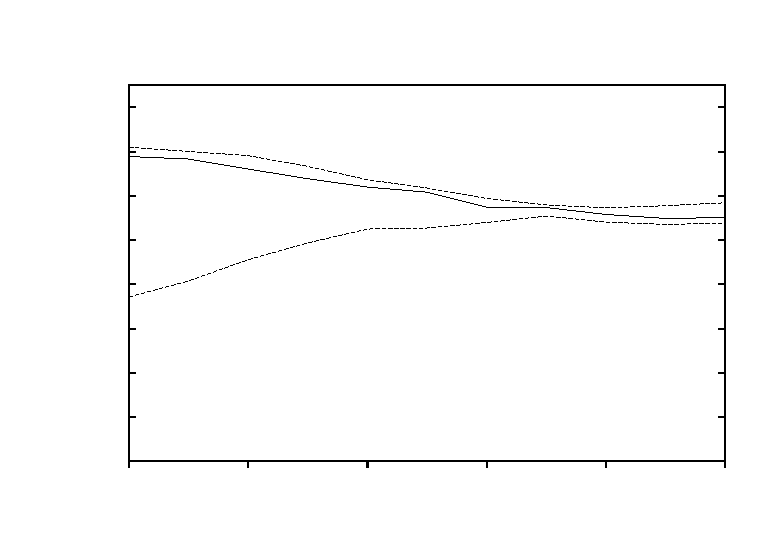
\includegraphics{zoav}}%
    \gplfronttext
  \end{picture}%
\endgroup
} & \resizebox{0.5\textwidth}{!}{% GNUPLOT: LaTeX picture with Postscript
\begingroup
  \makeatletter
  \providecommand\color[2][]{%
    \GenericError{(gnuplot) \space\space\space\@spaces}{%
      Package color not loaded in conjunction with
      terminal option `colourtext'%
    }{See the gnuplot documentation for explanation.%
    }{Either use 'blacktext' in gnuplot or load the package
      color.sty in LaTeX.}%
    \renewcommand\color[2][]{}%
  }%
  \providecommand\includegraphics[2][]{%
    \GenericError{(gnuplot) \space\space\space\@spaces}{%
      Package graphicx or graphics not loaded%
    }{See the gnuplot documentation for explanation.%
    }{The gnuplot epslatex terminal needs graphicx.sty or graphics.sty.}%
    \renewcommand\includegraphics[2][]{}%
  }%
  \providecommand\rotatebox[2]{#2}%
  \@ifundefined{ifGPcolor}{%
    \newif\ifGPcolor
    \GPcolorfalse
  }{}%
  \@ifundefined{ifGPblacktext}{%
    \newif\ifGPblacktext
    \GPblacktexttrue
  }{}%
  % define a \g@addto@macro without @ in the name:
  \let\gplgaddtomacro\g@addto@macro
  % define empty templates for all commands taking text:
  \gdef\gplbacktext{}%
  \gdef\gplfronttext{}%
  \makeatother
  \ifGPblacktext
    % no textcolor at all
    \def\colorrgb#1{}%
    \def\colorgray#1{}%
  \else
    % gray or color?
    \ifGPcolor
      \def\colorrgb#1{\color[rgb]{#1}}%
      \def\colorgray#1{\color[gray]{#1}}%
      \expandafter\def\csname LTw\endcsname{\color{white}}%
      \expandafter\def\csname LTb\endcsname{\color{black}}%
      \expandafter\def\csname LTa\endcsname{\color{black}}%
      \expandafter\def\csname LT0\endcsname{\color[rgb]{1,0,0}}%
      \expandafter\def\csname LT1\endcsname{\color[rgb]{0,1,0}}%
      \expandafter\def\csname LT2\endcsname{\color[rgb]{0,0,1}}%
      \expandafter\def\csname LT3\endcsname{\color[rgb]{1,0,1}}%
      \expandafter\def\csname LT4\endcsname{\color[rgb]{0,1,1}}%
      \expandafter\def\csname LT5\endcsname{\color[rgb]{1,1,0}}%
      \expandafter\def\csname LT6\endcsname{\color[rgb]{0,0,0}}%
      \expandafter\def\csname LT7\endcsname{\color[rgb]{1,0.3,0}}%
      \expandafter\def\csname LT8\endcsname{\color[rgb]{0.5,0.5,0.5}}%
    \else
      % gray
      \def\colorrgb#1{\color{black}}%
      \def\colorgray#1{\color[gray]{#1}}%
      \expandafter\def\csname LTw\endcsname{\color{white}}%
      \expandafter\def\csname LTb\endcsname{\color{black}}%
      \expandafter\def\csname LTa\endcsname{\color{black}}%
      \expandafter\def\csname LT0\endcsname{\color{black}}%
      \expandafter\def\csname LT1\endcsname{\color{black}}%
      \expandafter\def\csname LT2\endcsname{\color{black}}%
      \expandafter\def\csname LT3\endcsname{\color{black}}%
      \expandafter\def\csname LT4\endcsname{\color{black}}%
      \expandafter\def\csname LT5\endcsname{\color{black}}%
      \expandafter\def\csname LT6\endcsname{\color{black}}%
      \expandafter\def\csname LT7\endcsname{\color{black}}%
      \expandafter\def\csname LT8\endcsname{\color{black}}%
    \fi
  \fi
  \setlength{\unitlength}{0.0500bp}%
  \begin{picture}(7200.00,5040.00)%
    \gplgaddtomacro\gplbacktext{%
      \csname LTb\endcsname%
      \put(946,767){\makebox(0,0)[r]{\strut{} 0}}%
      \put(946,1192){\makebox(0,0)[r]{\strut{} 0.2}}%
      \put(946,1617){\makebox(0,0)[r]{\strut{} 0.4}}%
      \put(946,2042){\makebox(0,0)[r]{\strut{} 0.6}}%
      \put(946,2467){\makebox(0,0)[r]{\strut{} 0.8}}%
      \put(946,2892){\makebox(0,0)[r]{\strut{} 1}}%
      \put(946,3317){\makebox(0,0)[r]{\strut{} 1.2}}%
      \put(946,3742){\makebox(0,0)[r]{\strut{} 1.4}}%
      \put(946,4167){\makebox(0,0)[r]{\strut{} 1.6}}%
      \put(1078,484){\makebox(0,0){\strut{} 0}}%
      \put(2223,484){\makebox(0,0){\strut{} 0.1}}%
      \put(3368,484){\makebox(0,0){\strut{} 0.2}}%
      \put(4513,484){\makebox(0,0){\strut{} 0.3}}%
      \put(5658,484){\makebox(0,0){\strut{} 0.4}}%
      \put(6803,484){\makebox(0,0){\strut{} 0.5}}%
      \put(176,2573){\makebox(0,0){\strut{}$h$}}%
      \put(3940,154){\makebox(0,0){\strut{}$\alpha$}}%
      \put(3940,4709){\makebox(0,0){\strut{}$s_p$}}%
    }%
    \gplgaddtomacro\gplfronttext{%
    }%
    \gplbacktext
    \put(0,0){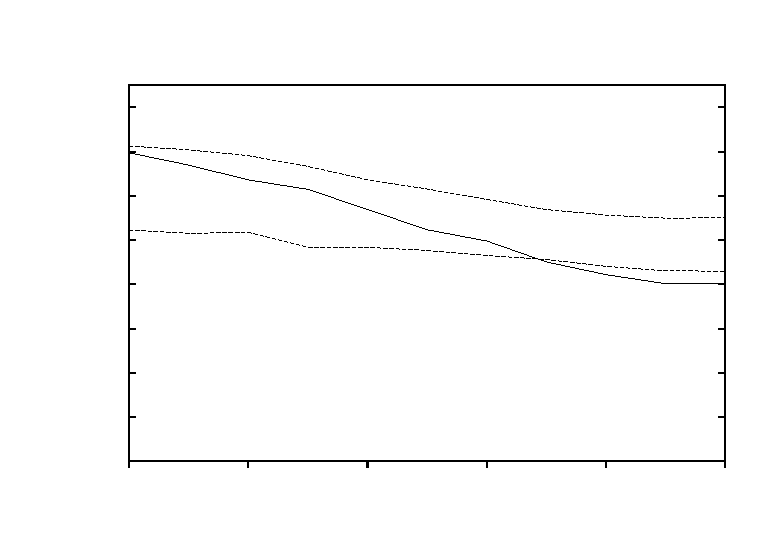
\includegraphics{zopop}}%
    \gplfronttext
  \end{picture}%
\endgroup
 }\\
(c) & (d) \\
\resizebox{0.5\textwidth}{!}{% GNUPLOT: LaTeX picture with Postscript
\begingroup
  \makeatletter
  \providecommand\color[2][]{%
    \GenericError{(gnuplot) \space\space\space\@spaces}{%
      Package color not loaded in conjunction with
      terminal option `colourtext'%
    }{See the gnuplot documentation for explanation.%
    }{Either use 'blacktext' in gnuplot or load the package
      color.sty in LaTeX.}%
    \renewcommand\color[2][]{}%
  }%
  \providecommand\includegraphics[2][]{%
    \GenericError{(gnuplot) \space\space\space\@spaces}{%
      Package graphicx or graphics not loaded%
    }{See the gnuplot documentation for explanation.%
    }{The gnuplot epslatex terminal needs graphicx.sty or graphics.sty.}%
    \renewcommand\includegraphics[2][]{}%
  }%
  \providecommand\rotatebox[2]{#2}%
  \@ifundefined{ifGPcolor}{%
    \newif\ifGPcolor
    \GPcolorfalse
  }{}%
  \@ifundefined{ifGPblacktext}{%
    \newif\ifGPblacktext
    \GPblacktexttrue
  }{}%
  % define a \g@addto@macro without @ in the name:
  \let\gplgaddtomacro\g@addto@macro
  % define empty templates for all commands taking text:
  \gdef\gplbacktext{}%
  \gdef\gplfronttext{}%
  \makeatother
  \ifGPblacktext
    % no textcolor at all
    \def\colorrgb#1{}%
    \def\colorgray#1{}%
  \else
    % gray or color?
    \ifGPcolor
      \def\colorrgb#1{\color[rgb]{#1}}%
      \def\colorgray#1{\color[gray]{#1}}%
      \expandafter\def\csname LTw\endcsname{\color{white}}%
      \expandafter\def\csname LTb\endcsname{\color{black}}%
      \expandafter\def\csname LTa\endcsname{\color{black}}%
      \expandafter\def\csname LT0\endcsname{\color[rgb]{1,0,0}}%
      \expandafter\def\csname LT1\endcsname{\color[rgb]{0,1,0}}%
      \expandafter\def\csname LT2\endcsname{\color[rgb]{0,0,1}}%
      \expandafter\def\csname LT3\endcsname{\color[rgb]{1,0,1}}%
      \expandafter\def\csname LT4\endcsname{\color[rgb]{0,1,1}}%
      \expandafter\def\csname LT5\endcsname{\color[rgb]{1,1,0}}%
      \expandafter\def\csname LT6\endcsname{\color[rgb]{0,0,0}}%
      \expandafter\def\csname LT7\endcsname{\color[rgb]{1,0.3,0}}%
      \expandafter\def\csname LT8\endcsname{\color[rgb]{0.5,0.5,0.5}}%
    \else
      % gray
      \def\colorrgb#1{\color{black}}%
      \def\colorgray#1{\color[gray]{#1}}%
      \expandafter\def\csname LTw\endcsname{\color{white}}%
      \expandafter\def\csname LTb\endcsname{\color{black}}%
      \expandafter\def\csname LTa\endcsname{\color{black}}%
      \expandafter\def\csname LT0\endcsname{\color{black}}%
      \expandafter\def\csname LT1\endcsname{\color{black}}%
      \expandafter\def\csname LT2\endcsname{\color{black}}%
      \expandafter\def\csname LT3\endcsname{\color{black}}%
      \expandafter\def\csname LT4\endcsname{\color{black}}%
      \expandafter\def\csname LT5\endcsname{\color{black}}%
      \expandafter\def\csname LT6\endcsname{\color{black}}%
      \expandafter\def\csname LT7\endcsname{\color{black}}%
      \expandafter\def\csname LT8\endcsname{\color{black}}%
    \fi
  \fi
  \setlength{\unitlength}{0.0500bp}%
  \begin{picture}(7200.00,5040.00)%
    \gplgaddtomacro\gplbacktext{%
      \csname LTb\endcsname%
      \put(946,767){\makebox(0,0)[r]{\strut{} 0}}%
      \put(946,1239){\makebox(0,0)[r]{\strut{} 0.2}}%
      \put(946,1710){\makebox(0,0)[r]{\strut{} 0.4}}%
      \put(946,2182){\makebox(0,0)[r]{\strut{} 0.6}}%
      \put(946,2653){\makebox(0,0)[r]{\strut{} 0.8}}%
      \put(946,3125){\makebox(0,0)[r]{\strut{} 1}}%
      \put(946,3596){\makebox(0,0)[r]{\strut{} 1.2}}%
      \put(946,4068){\makebox(0,0)[r]{\strut{} 1.4}}%
      \put(946,4539){\makebox(0,0)[r]{\strut{} 1.6}}%
      \put(1078,484){\makebox(0,0){\strut{} 0}}%
      \put(2223,484){\makebox(0,0){\strut{} 0.1}}%
      \put(3368,484){\makebox(0,0){\strut{} 0.2}}%
      \put(4513,484){\makebox(0,0){\strut{} 0.3}}%
      \put(5658,484){\makebox(0,0){\strut{} 0.4}}%
      \put(6803,484){\makebox(0,0){\strut{} 0.5}}%
      \put(176,2771){\makebox(0,0){\strut{}$h$}}%
      \put(3940,154){\makebox(0,0){\strut{}$\alpha$}}%
    }%
    \gplgaddtomacro\gplfronttext{%
    }%
    \gplbacktext
    \put(0,0){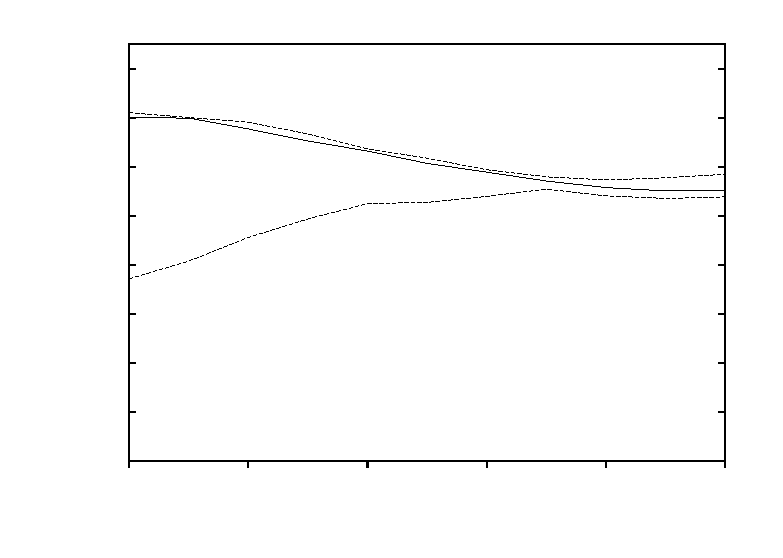
\includegraphics{zhav}}%
    \gplfronttext
  \end{picture}%
\endgroup
 } & \resizebox{0.5\textwidth}{!}{% GNUPLOT: LaTeX picture with Postscript
\begingroup
  \makeatletter
  \providecommand\color[2][]{%
    \GenericError{(gnuplot) \space\space\space\@spaces}{%
      Package color not loaded in conjunction with
      terminal option `colourtext'%
    }{See the gnuplot documentation for explanation.%
    }{Either use 'blacktext' in gnuplot or load the package
      color.sty in LaTeX.}%
    \renewcommand\color[2][]{}%
  }%
  \providecommand\includegraphics[2][]{%
    \GenericError{(gnuplot) \space\space\space\@spaces}{%
      Package graphicx or graphics not loaded%
    }{See the gnuplot documentation for explanation.%
    }{The gnuplot epslatex terminal needs graphicx.sty or graphics.sty.}%
    \renewcommand\includegraphics[2][]{}%
  }%
  \providecommand\rotatebox[2]{#2}%
  \@ifundefined{ifGPcolor}{%
    \newif\ifGPcolor
    \GPcolorfalse
  }{}%
  \@ifundefined{ifGPblacktext}{%
    \newif\ifGPblacktext
    \GPblacktexttrue
  }{}%
  % define a \g@addto@macro without @ in the name:
  \let\gplgaddtomacro\g@addto@macro
  % define empty templates for all commands taking text:
  \gdef\gplbacktext{}%
  \gdef\gplfronttext{}%
  \makeatother
  \ifGPblacktext
    % no textcolor at all
    \def\colorrgb#1{}%
    \def\colorgray#1{}%
  \else
    % gray or color?
    \ifGPcolor
      \def\colorrgb#1{\color[rgb]{#1}}%
      \def\colorgray#1{\color[gray]{#1}}%
      \expandafter\def\csname LTw\endcsname{\color{white}}%
      \expandafter\def\csname LTb\endcsname{\color{black}}%
      \expandafter\def\csname LTa\endcsname{\color{black}}%
      \expandafter\def\csname LT0\endcsname{\color[rgb]{1,0,0}}%
      \expandafter\def\csname LT1\endcsname{\color[rgb]{0,1,0}}%
      \expandafter\def\csname LT2\endcsname{\color[rgb]{0,0,1}}%
      \expandafter\def\csname LT3\endcsname{\color[rgb]{1,0,1}}%
      \expandafter\def\csname LT4\endcsname{\color[rgb]{0,1,1}}%
      \expandafter\def\csname LT5\endcsname{\color[rgb]{1,1,0}}%
      \expandafter\def\csname LT6\endcsname{\color[rgb]{0,0,0}}%
      \expandafter\def\csname LT7\endcsname{\color[rgb]{1,0.3,0}}%
      \expandafter\def\csname LT8\endcsname{\color[rgb]{0.5,0.5,0.5}}%
    \else
      % gray
      \def\colorrgb#1{\color{black}}%
      \def\colorgray#1{\color[gray]{#1}}%
      \expandafter\def\csname LTw\endcsname{\color{white}}%
      \expandafter\def\csname LTb\endcsname{\color{black}}%
      \expandafter\def\csname LTa\endcsname{\color{black}}%
      \expandafter\def\csname LT0\endcsname{\color{black}}%
      \expandafter\def\csname LT1\endcsname{\color{black}}%
      \expandafter\def\csname LT2\endcsname{\color{black}}%
      \expandafter\def\csname LT3\endcsname{\color{black}}%
      \expandafter\def\csname LT4\endcsname{\color{black}}%
      \expandafter\def\csname LT5\endcsname{\color{black}}%
      \expandafter\def\csname LT6\endcsname{\color{black}}%
      \expandafter\def\csname LT7\endcsname{\color{black}}%
      \expandafter\def\csname LT8\endcsname{\color{black}}%
    \fi
  \fi
  \setlength{\unitlength}{0.0500bp}%
  \begin{picture}(7200.00,5040.00)%
    \gplgaddtomacro\gplbacktext{%
      \csname LTb\endcsname%
      \put(946,767){\makebox(0,0)[r]{\strut{} 0}}%
      \put(946,1239){\makebox(0,0)[r]{\strut{} 0.2}}%
      \put(946,1710){\makebox(0,0)[r]{\strut{} 0.4}}%
      \put(946,2182){\makebox(0,0)[r]{\strut{} 0.6}}%
      \put(946,2653){\makebox(0,0)[r]{\strut{} 0.8}}%
      \put(946,3125){\makebox(0,0)[r]{\strut{} 1}}%
      \put(946,3596){\makebox(0,0)[r]{\strut{} 1.2}}%
      \put(946,4068){\makebox(0,0)[r]{\strut{} 1.4}}%
      \put(946,4539){\makebox(0,0)[r]{\strut{} 1.6}}%
      \put(1078,484){\makebox(0,0){\strut{} 0}}%
      \put(2223,484){\makebox(0,0){\strut{} 0.1}}%
      \put(3368,484){\makebox(0,0){\strut{} 0.2}}%
      \put(4513,484){\makebox(0,0){\strut{} 0.3}}%
      \put(5658,484){\makebox(0,0){\strut{} 0.4}}%
      \put(6803,484){\makebox(0,0){\strut{} 0.5}}%
      \put(176,2771){\makebox(0,0){\strut{}$h$}}%
      \put(3940,154){\makebox(0,0){\strut{}$\alpha$}}%
    }%
    \gplgaddtomacro\gplfronttext{%
    }%
    \gplbacktext
    \put(0,0){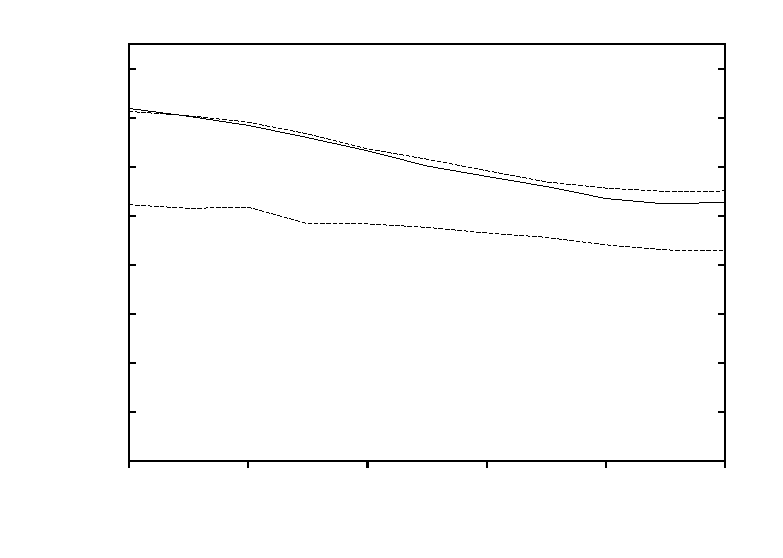
\includegraphics{zhpop}}%
    \gplfronttext
  \end{picture}%
\endgroup
}
\end{tabular}
\bigskip
\rule{33em}{0.5pt}
\caption{ \label{zeroone} Above is the performance of the adaptive multi-unit ISI metrics.  (a) $s_a$ with population parameter $p$ at each instant set to one if $s(t)<0.5$ and set to zero otherwise. (b) $s_p$ with population parameter $p$ at each instant set to one if $s(t)<0.5$ and set to zero otherwise. (c) $s_a$ with population parameter $p$ at each instant set to 0.5 if $s(t)<0.5$ and set to zero otherwise. (d) $s_p$ with population parameter $p$ at each instant set t0 0.5 if $s(t)<0.5$ and set to zero otherwise.}
\end{center}
\end{figure}

